\ssection[Samandrag]{Samandrag}

\begin{multicols}{2}

I løpet av dei siste 60 åra har Europa utvikla ein eigen politisk og økonomisk struktur. Likevel er det framleis ein stor kulturell og språkleg variasjon. Frå portugisisk til polsk og italiensk til islandsk møter ein språkbarrierar, så vel i vanleg kommunikasjon mellom europeiske innbyggjarar som i handel og politikk. EU-institusjonane bruker årleg rundt ein milliard euro på å støtte den fleirspråklege politikken, til dømes gjennom omsetjing av tekst og tolking av talt kommunikasjon. Men er det naudsynt med ei slik byrde? Moderne språkteknologi og lingvistisk forsking kan gje eit viktig bidrag til å rive ned murane mellom språk. Kombinert med intelligente verktøy og applikasjonar kan språkteknologi hjelpe europearar i kommunikasjon og handel med kvarandre, sjølv om dei ikkje snakkar eit felles språk. 

\boxtext{Språkteknologi byggjer bruer.}

Noreg har ein eksportbasert økonomi og er i tillegg tungt involvert i internasjonale humanitære, diplomatiske og militære aktivitetar. Difor er gode språkkunnskapar, både i engelsk og andre framandspråk, essensielle for nordmenn.
Likevel kan språkbarrierar vere eit hinder for handel, spesielt for små og mellomstore føretak som ikkje har dei økonomiske midlane til å dekkje behovet. Det einaste (utenkjelege) alternativet til vårt noverande, fleirspråklege Europa ville vere å la eit enkelt språk overta ein dominant posisjon og ende opp med å erstatte alle andre språk. 

Ein klassisk strategi for å kome over språkbarrieren er å lære framandspråk. Utan teknisk støtte er det ei overveldande oppgåve å prøve å dekkje alle 23 offisielle språk og omtrent 60 andre europeiske språk, både for einskildpersonar, næringslivet, politisk debatt og vitskapleg verksemd. 

Løysinga er å byggje ut nøkkelteknologiar. Desse vil gje europeiske aktørar enorme fordelar, ikkje berre innanfor den felles europeiske marknaden, men òg i handelsrelasjonar med andre land, spesielt land med veksande økonomiar. For å oppnå dette målet og verne Europas kulturelle og språklege mangfald, er det første steget systematisk å analysere dei språklege særtrekka, og dermed utfordringane, for alle europeiske språk. Dinest treng vi eit oversyn over den noverande tilstanden for språkteknologisk støtte for dei ulike språka. Språkteknologiske løysingar vil etter kvart fungere som ei unik bru mellom språka i Europa. 
    
Dagens verktøy for automatisk omsetjing og taleprosessering strekkjer ikkje til for å nå dette ambisiøse målet. Dei dominerande aktørane på dette området er for det meste privatåtte kommersielle selskap i Nord-Amerika. Alt på slutten av 1970-talet føresåg EU at språkteknologi verkeleg kunne bli ein motor for europeisk eining, og byrja då å finansiere dei første store forskingsprosjekta i Europa, som t.d. EUROTRA. Samstundes vart òg nasjonale prosjekt gradvis etablerte. Dei leverte verdifulle resultat, men førde aldri til ein klårt samkøyrd europeisk innsats. I motsetnad til denne selektive finansieringsinnsatsen i Europa har andre fleirspråklege samfunn som India (med sine 22 offisielle språk) og Sør-Afrika (med sine 11 offisielle språk) nyleg initiert langsiktige nasjonale program for språkforsking og teknologiutvikling. 

Dei dominerande aktørane innanfor språkteknologi er i dag avhengige av upresise statistiske tilnærmingar som ikkje nyttar djupare lingvistisk kunnskap og metodar. Setningar blir vanlegvis omsette automatisk ved å samanlikne ei ny setning med tusenvis av setningar som tidlegare er omsette av menneske (eit treningsdatasett). Omsetjingskvaliteten avheng i stor grad av mengda og kvaliteten på det tilgjengelege treningsdatasettet som systemet kan lære frå. Medan automatisk omsetjing av enkle setningar i språk med tilstrekkelege mengder treningsmateriale kan gje brukande resultat, kan ikkje statistiske tilnærmingar bli like vellukka for språk som har ei betydeleg mindre mengd treningsmateriale eller for setningar med komplekse strukturar. Desse krev ein djupare lingvistisk analyse. Analysar av dei djupare, strukturelle trekka i språka er den einaste løysinga for å byggje applikasjonar som fungerer godt for alle dei europeiske språka.

\boxtext{Språkteknologi som ein nykel for framtida.}

Difor har EU vedteke å finansiere prosjekt som EuroMatrix og EuroMatrixPlus (med oppstart i 2006) og iTranslate4 (med oppstart i 2010), som driv grunnforsking og bruksretta forsking, og som byggjer ressursar retta mot språkteknologiske løysingar av høg kvalitet for alle europeiske språk. Ein djupare analyse av strukturelle eigenskapar ved språk er den einaste vegen framover om vi ynskjer å byggje applikasjonar som gjev gode resultat på tvers av heile spektret av Europas språk. 
I europeisk samanheng har ein alt oppnådd ei rekkje gode resultat innanfor forsking på dette området. Til dømes bruker omsetjingstenester i EU no MOSES, ei programvare med open kjeldekode for maskinomsetjing som i hovudsak er utvikla i europeiske forskingsprosjekt. Prosjektet Verbmobil, finansiert av det tyske Utdannings- og forskingsdepartementet (BMBF) mellom 1993 og 2000, sette Tyskland i tet innanfor taleomsetjingsforsking i ein periode. Mange forskings- og utviklingslaboratorium som var aktive i Tyskland på den tida (til dømes IBM og Philips), har sidan vorte nedlagde eller flytta. Snarare enn å byggje på resultata av forskinga si, har Europa ein tendens til å forfølgje isolerte og kortvarige forskingsaktivitetar med avgrensa påverknad på marknaden.

Det økonomiske verdet av tidleg innsats kan mælast i mengder sideverknader. Norske TextUrgy vart etablert i 2007 og har utvikla ei løysing for å gje betre søkeresultat basert på forskingsarbeid. Dei har brukt tida på å utvikle løysinga si, som først no er moden for kommersialisering. 

\boxtext{Språkteknologi forenklar kommunikasjon i Europa}

I dag står dagens `hybrid'-språkteknologi fram som ei lovande blanding av djup lingvistisk analyse med grunne statistiske metodar. Slike system kan byggje bruer mellom språk. META-NETs serie av språkrapportar viser at det er ein dramatisk skilnad på beredskapsnivået mellom dei europeiske landa når det gjeld tilgjengelege språkteknologiske løysingar og kor langt forskinga har kome. 

Denne rapporten om situasjonen for det norske språket viser at norsk på den eine sida har ein trygg posisjon som både nasjonal- og majoritetsspråk. Informasjons- og kommunikasjonsteknologi (IKT) er i bruk på alle samfunnsområde og 93\% av den norske folkesetnaden har tilgang til Internett. 

På den andre sida blir ikkje denne generelt gode IKT-situasjonen følgd opp av ein tilsvarande tilfredsstillande status for Forsking og Utvikling (FoU) innan språkressursar og -teknologi (SRT). Utviklinga av språkteknologiske produkt føreset visse grunnleggjande data (ordlister, tekstkorpus, talekorpus). Både dei grunnleggjande språkressursane, og produkt som blir utvikla på grunnlag av dei, er like kostbare og tidkrevjande å utvikle for mindre språk som for større språk. Sidan norsk har to offisielle skriftlege normer og mange dialektar, er utviklingskostnadene endå høgare. Løysingar for norsk er difor ikkje kommersielt attraktive, og er i stor grad avhengig av offentleg finansiering. 

Gjennom ein felles innsats frå Språkrådet, Forskingsrådet, kommersielle aktørar og norske forskingsinstitusjonar er det i dag er eit gryande politisk medvit om at språkteknologi er viktig for at Noreg enno skal kunne hevde seg ikkje berre industrielt, men òg kulturelt. 
Dette auka medvitet har ført til to viktige milestolpar i utviklinga av norsk SRT: Forskingsprogrammet KUNSTI og etablering av \textit{Språkteknologisk ressurssamling for norsk – Språkbanken}.
Den første milestolpen var KUNSTI, det første koordinerte norske forskingsprogrammet som var spesielt retta mot norsk SRT (2001–2006). Det vart starta tjue forskingsprosjekt som fostra nye forskarar og skapte einskilde grunnleggjande språkressursar og verktøy for norsk, men svært få av desse vart gjorde tilgjengelege for generell gjenbruk i vidare forsking og utvikling.
Den andre milestolpen vart \textit{Språkteknologisk ressurssamling for norsk – Språkbanken}, etablert i 2010, etter å ha vore på dagsorden i to tiår. Språkbanken skal fungere som ein infrastruktur for å gjere norsk SRT tilgjengeleg for forsking og kommersiell utvikling, og vil dimed – vonleg – senke terskelen for å utvikle norske SRT-produkt. 

Denne kvitboka viser at norsk enno ikkje har på langt nær eit så tilfredsstillande utval av språkteknologiske applikasjonar av høg kvalitet som engelsk. Grunnleggjande SRT-ar finst for norsk, men i nokre tilfelle er dei ufullstendige. Ofte er det restriksjonar på bruk, og ofte har dei manglande kompatibilitet og mangelfull dokumentasjon. Vidare er mange forskingsresultat ikkje tilstrekkeleg godt kjende, og mange potensielle brukarar kjenner ikkje til desse funna. Der er òg framleis klåre behov, blant anna for ein nasjonal infrastruktur for terminologi, parallellkorpus av tilstrekkeleg storleik, og korpus av spontan tale med ei god dialektdekning. 

Hos leverandørar av språktenester synest det å vere eit underforbruk av SRT for norsk. 
Potensielle brukarar av SRT er ofte klår over dei moglege fordelane, men dei har ikkje kompetanse til å ta i bruk slike system sjølv, og dei finn det vanskeleg å vurdere føremonane av tilgjengelege LRT. Difor har vi enno ein lang veg å gå for å sikre det norske språket i det digitale informasjonssamfunnet. 

META-NET sitt langsiktige mål er å formidle språkteknologi av høg kvalitet til alle språka i Europa, for å skape politisk og økonomisk samarbeid på tvers av landegrenser og kulturelt mangfald. Denne teknologien kan bidra til å fjerne barrierar og til å byggje bruer mellom dei europeiske språka. Dette krev at alle interessentar – i politikk, forsking, næringslivet og samfunnet som heilskap – står saman i ein felles innsats for framtida.

Denne rapportserien kjem i tillegg til META-NETs andre strategiske tiltak (sjå appendiks for eit oversyn). Oppdatert informasjon om til dømes META-NET sitt Visjonsdokument  \cite{Meta1} eller den Strategiske forskingsagendaen finst på META-NET si nettside, \url{http://www.meta-net.eu}.
\end{multicols}

\clearpage

\ssection[Språka våre står i fare]{Språka våre står i fare: Ei utfordring for språkteknologien 
}

\begin{multicols}{2}

Vi er vitne til ein digital revolusjon som påverkar kommunikasjonen og samfunnet dramatisk. Den seinaste utviklinga i digital informasjons- og kommunikasjonsteknologi blir nokre gonger samanlikna med Gutenbergs oppfinning av trykkpressa. Kva kan denne analogien fortelje oss om framtida for det europeiske informasjonssamfunnet generelt og for stillinga til språka spesielt? 

\boxtext{Vi er vitne til ein digital revolusjon som kan samanliknast med Gutenbergs oppfinning av trykkpressa.}

I kjølvatnet av Gutenbergs oppfinning skjedde fleire store gjennombrot i kommunikasjon og kunnskapsutveksling, som til dømes Luthers omsetjing av Bibelen til eige morsmål. Sidan Gutenbergs tid har ein utvikla fleire teknikkar for betre handsaming av språkbehandling og kunnskapsutveksling: 

\begin{itemize}
\item standardisering av rettskriving og grammatikk for dei vanlegaste språka har gjeve ei hurtigare spreiing av nye vitskaplege og intellektuelle idear;
\item utviklinga av offisielle språk har gjort det lettare for innbyggjarane å kommunisere innanfor visse (som oftast politiske) grenser; 
\item undervising og omsetjing mellom språk har bidrege til utveksling på tvers av språk; 
\item  etablering av redaksjonelle og bibliografiske retningsliner har sikra kvaliteten og tilgangen på trykt materiale; 
\item etablering av ulike medium som aviser, radio, fjernsyn, bøker og andre medium har dekt ei rekkje kommunikasjonsbehov. 
\end{itemize}

Dei siste tjue åra har informasjonsteknologi bidrege til å automatisere og forenkle mange av desse prosessane: 

\begin{itemize}
\item publiserings- og teksthandsamingsprogram har erstatta skrivemaskin og dokumentproduksjon; 
\item Microsoft PowerPoint har erstatta overheadtransparentar; 
\item e-post gjer det mogleg å sende og ta mot dokument raskare enn med ei faksmaskin; 
\item Skype tilbyr billege telefonsamtaler via Internett og legg til rette for videokonferansar; 
\item ulike format for lagring av lydar og video gjer det enkelt å utveksle multimedie-innhald; 
\item søkemotorar gjer det enkelt å søkje i nettsider; 
\item nettbaserte tenester som Google Translate produserer raske, omtrentlege omsetjingar; 
\item sosiale medium som Facebook, Twitter og Google + forenklar hurtig kommunikasjon, samarbeid og informasjonsdeling. 
\end{itemize}

Sjølv om slike verktøy og program er nyttige, er dei enno ikkje i stand til fullt ut å fylle rolla som ein berebjelke for innbyggjarane i eit fleirspråkleg europeisk samfunn, med fri flyt av informasjon og varer. 

\subsection[Språkgrenser hindrar utviklinga av eit europeisk informasjonssamfunn ]{Språkgrenser hindrar utviklinga av eit europeisk informasjonssamfunn }

Vi kan ikkje føreseie nøyaktig korleis informasjonssamfunnet vil sjå ut i framtida. Men det er svært sannsynleg at den viktigaste revolusjonen i moderne kommunikasjonsteknologi vil liggje i nye måtar å samle folk som snakkar ulike språk. Dette legg press på den einskilde, som må lære nye språk, og på programutviklarar, som må lage nye applikasjonar som kan sikre gjensidig forståing og tilgjenge til deleleg kunnskap. I ein økonomi og eit informasjonssamfunn som blir stadig meir globalisert, vil nye medium føre til enklare interaksjon på tvers av språk, språkbrukarar og ulike typar innhald. Sosiale medium som Wikipedia, Facebook, Twitter, YouTube, og nyleg Google+ har vorte stadig meir utbreidde, men dette er berre toppen av isfjellet.

\boxtext{Ein stadig meir globalisert økonomi og informasjonssamfunn konfronterer oss med fleire språk, ulike språkbrukarar og ulike typar innhald.}

Ifølgje ein fersk rapport frå Europakommisjonen kjøper 57\% av Internettbrukarane i Europa varar og tenester på språk som ikkje er deira eige morsmål (engelsk er det vanlegaste framandspråket, følgd av fransk, tysk og spansk). 55\% av brukarane kan lese innhald på eit framandspråk, medan berre 35\% bruker eit anna språk til å skrive e-post eller poste kommentarar på nettet \cite{EC1}. For nokre år sidan var kanskje engelsk Internettet sitt \textit{lingua franca}, men no er situasjonen dramatisk forandra. Mengda av nettbasert innhald på andre europeiske språk (og dessutan asiatiske og språk frå Midtausten) har eksplodert. 

Denne digitale 'klasseskilnaden' mellom språka har overraskande nok ikkje fått mykje offentleg merksemd, trass i at det gjennomsyrar heile samfunnet. Men det aktualiserer eit viktig spørsmål: Kva for europeiske språk vil overleve i eit nettverksbasert informasjons- og kunnskapssamfunn, og kva for språk er dømde til å forsvinne?

\subsection{Språka våre står i fare}

Medan trykkjeteknologien bidrog til å auke informasjonsspreiinga i Europa, førde han òg til språkdød. Regionale og minoritetsspråk vart sjeldan trykte, slik at språk som kornisk og dalmatisk vart avgrensa til munnleg overføring, noko som i sin tur avgrensa bruksområda. Vil Internett har same verknad på språka våre?

\boxtext{Det språklege mangfaldet i Europa er ein av dei viktigaste delane av kulturarven vår.}

Dei om lag 80 språka i Europa utgjer ein av dei viktigaste delane av kulturarven vår, og ein sentral del av den europeiske samfunnsmodellen \cite{EC2}. Medan språk som engelsk og spansk sannsynlegvis vil overleve på den nye digitale marknaden, risikerer mange europeiske språk å bli irrelevante i eit nettverksbasert samfunn. Dette ville kunne svekkje Europas posisjon på verdsbasis og svekkje målet om likeverdig deltaking for alle europeiske borgarar, uavhengig av språk. Ifølgje ein UNESCO-rapport om fleirspråklegheit er språk eit viktig middel for å nyte godt av grunnleggjande rettar, som politisk ytringsfridom, utdanning og samfunnsdeltaking  \cite{Unesco1}. 

\subsection{Språkteknologi kan leggje til rette for språkbruk}

Tidlegare vart det først og fremst investert i språkopplæring og omsetjing. Utrekningar viser at den europeiske marknaden for omsetjing, tolking, programvarelokalisering og nettstadsglobalisering utgjorde 8,4 milliardar euro i 2008, og dette talet blir forventa å vekse med 10\% årleg \cite{EC3}. Men denne investeringa dekkjer berre ein liten del av det noverande og framtidige behovet for kommunikasjon mellom språk. Eit viktig tiltak for å sikre breidda og mangfaldet av språkbruk i morgondagens Europa er å bruke riktig teknologi, akkurat som vi bruker teknologi til å løyse utfordringar innan transport, energi og universell utforming. 

Digital språkteknologi (retta mot alle former for tekst og munnleg tale) kan hjelpe menneske til å samarbeide, drive handel, dele kunnskap og delta i sosiale og politiske debattar på tvers av språkbarrierar og datakunnskapar. Språkteknologi er ofte innebygd i komplekse system som hjelper oss med å: 

\begin{itemize}
\item finne informasjon med ein Internett-søkemotor; 
\item sjekke staving og grammatikk i eit teksthandsamingsprogram; 
\item vise produkttilrådingane i nettbutikkar; 
\item høyre taleinstruksjonar frå eit bilnavigasjonssystem; 
\item omsetje nettsider via nettbaserte tenester. 
\end{itemize}

Språkteknologi består av ei rekkje kjerneapplikasjonar som legg til rette for ulike prosessar innanfor eit større applikasjonsrammeverk. Føremålet med META-NETs språkrapportar er å undersøkje i kva grad og kor godt desse kjerneteknologiane er utvikla for dei europeiske språka. 

\boxtext{Vi treng robust og rimeleg språkteknologi for alle dei europeiske språka.}

For å oppretthalde ein leiande posisjon i global innovasjon treng Europa ein språkteknologi som er tilpassa alle europeiske språk og som er robust, rimeleg og tett integrert i relevant programvare. Utan språkteknologi vil vi ikkje kunne skape ei effektiv, interaktiv, multimedial og fleirspråkleg brukaroppleving i den nære framtida.

\subsection{Språkteknologi gjev moglegheiter.}

I ei verd basert på trykkjeteknologi var det viktige teknologiske gjennombrotet rask kopiering av ei tekstside ved hjelp av ei trykkpresse. Det omstendelege arbeidet med å slå opp, lese, omsetje og oppsummere kunnskap måtte framleis utførast av menneske. Ikkje før Edison kunne ein lagre tale, og då berre som analoge kopiar. 

Digital språkteknologi kan no automatisere sjølve omsetjingsprosessen, innhaldsproduksjon og kunnskapshandsaming for alle europeiske språk. Språkteknologi kan òg bidra til intuitive talestyrte grensesnitt for hushaldningsmaskiner, bilar, datamaskiner og robotar. Vi er enno på eit tidleg stadium av utviklinga av å bruke kommersielle og industrielle applikasjonar, men FoU har skapt mange nye høve. Til dømes er maskinomsetjing alt vorten rimeleg nøyaktig innanfor visse område, og eksperimentelle applikasjonar mogleggjer fleirspråkleg informasjons- og kunnskapsstyring og dessutan innhaldsproduksjon for mange europeiske språk. 

Som med dei fleste teknologiane vart den første bruken innan bl.a. talebaserte brukargrensesnitt og dialogsystem utvikla for svært spesialiserte domene, og dei hadde ofte ei nokså avgrensa yting. Men det ligg store marknadspotensial innanfor utdanningssektoren og underhaldningsindustrien ved å integrere språkteknologi i spel, kulturminnestader, skule og anna opplæring, bibliotek, osb. Mobile informasjonstenester, datastøtta språklæring, eLæringsmiljø, eigenvurderingsverktøy og plagiatkontrollprogram er berre nokre av bruksområda der språkteknologi kan spele ei viktig rolle. Populariteten til sosiale medium som Twitter og Facebook illustrerer behovet for avanserte språkteknologiar som kan overvake innlegg, oppsummere diskusjonar, analysere meiningstrendar, oppdage kjenslereaksjonar, identifisere brot på lover og reglar eller spore misbruk.

\boxtext{Språkteknologi kan bidra til å bryte ned språkbarrierane som det språklege mangfaldet skaper.}

Språkteknologi representerer eit enormt potensial for EU. Han kan bidra til å handtere fleirspråklegheit i Europa – det faktumet at ulike språk lever i naturleg sameksistens i europeiske føretak, organisasjonar og skular. Men innbyggjarane treng å kommunisere på tvers av desse språkgrensene og på kryss og tvers av den felles europeiske marknaden. Språkteknologi kan bidra til å overvinne denne siste barrieren samstundes som han støttar fri og open bruk av det einskilde språket. Ser ein lenger framover, vil ein nyskapande og fleirspråkleg europeisk språkteknologi gje ein målestokk for dei globale partnarane våre når dei utviklar sine eigne fleirspråklege samfunn. Språkteknologi er ei form for 'hjelpemiddel'-teknologi som hjelper oss å bryte ned språklege barrierar og gjere språksamfunn meir tilgjengelege for kvarandre. 
Eit anna viktig og aktivt forskingsfelt er nytta av språkteknologi i redningsoperasjonar i katastrofeområde, der teknologiyting kan bli eit spørsmål om liv og død: Framtida sine intelligente robotar med tverrspråklege funksjonar kan redde liv. 
 
\subsection{Utfordringar for språkteknologi}

Sjølv om språkteknologien har gjort betydelege framsteg dei siste åra, skjer den noverande teknologiske utviklinga og produktinnovasjonen for sakte. Vanlege verktøy som stave- og grammatikkontroll i tekstbehandling er vanlegvis einspråklege og berre tilgjengelege for ei handfull språk. Nettbaserte maskinomsetjingstenester er nyttige for å få eit rask oversyn over innhaldet i dokumentet, men gjev store problem når svært nøyaktige og fullstendige omsetjingar trengst. På grunn av kompleksiteten i menneskeleg språk er det å modellere naturleg språkbruk i programvare for deretter å teste det ut i den verkelege verda ein tidkrevjande og kostbar operasjon som krev ei stabil finansiering. Dei europeiske landa må difor vere aktive i møte med dei teknologiske utfordringane eit fleirspråkleg samfunn står overfor gjennom aktivt å utvikle nye metodar for å skunde på utviklinga. Dette kan vere både utrekningsorienterte framsteg og teknikkar som 'crowdsourcing'.

\boxtext{Den teknologiske utviklinga går for langsamt.}

\subsection{Språktileigning hos menneske og maskiner}

For å illustrere korleis datamaskiner handterer naturleg språk, og kvifor det er vanskeleg å programmere dei til å prosessere ulike språk, skal vi kort sjå på korleis menneske tileignar seg første- og andrespråk, og deretter sjå korleis språkteknologiske system fungerer.

Menneske tileignar seg språkkunnskap på to ulike måtar. Babyar lærer eit språk ved å lytte til samspel mellom foreldre, sysken og andre familiemedlemmer. Frå toårsalderen produserer born dei første orda sine og korte setningar. Dette er berre mogleg fordi menneske har ein genetisk disposisjon til å imitere og rasjonalisere på grunnlag av det dei høyrer.

Å lære eit andrespråk på eit seinare stadium krev meir innsats, hovudsakleg fordi barnet ikkje er omgjeve av ein språkfellesskap, slik det er tilfelle for morsmålet. På skulen tileignar ein seg vanlegvis framandspråk gjennom å innarbeide grammatiske strukturar, ordtilfang og staving. Dette skjer ved hjelp av puggeøvingar som skildrar språklege kunnskapar gjennom abstrakte reglar, tabellar og døme.

\boxtext{Menneske tileignar seg språkkunnskap på to ulike måtar: Læring frå døme og læring frå underliggjande språkreglar.}

Dei to hovudtypane av språkteknologiske system `tileignar' seg språklege kunnskapar på ein liknande måte. Statistiske (eller `datadrivne') tilnærmingar innhentar språkkunnskap frå store samlingar av konkrete eksempeltekster. For å trene stavekontrollsystem er det tilstrekkeleg å bruke tekst frå eit enkelt språk, men skal ein trene opp eit maskinomsetjingssystem, treng ein eit sett av parallelle tekster for to (eller fleire) språk. På denne måten kan maskina `lære' mønster for korleis ord, korte setningar og fullstendige setningar blir omsette.

Ei statistisk tilnærming kan krevje millionar av setningar, og kvaliteten aukar jo meir tekst som blir analysert. Dette er ein av grunnane til at søkemotorleverandørar vil samle inn så mykje tekst som mogleg. Tekstbehandlingsprogramma sine stavekontrollar, så vel som tenester som Google Search og Google Translate, er alle baserte på statistiske metodar. Den store fordelen med statistiske metodar er at maskina lærer raskt gjennom ein kontinuerleg serie av treningsrundar, men kvaliteten er varierande.

Den andre tilnærminga til språkteknologi, og særleg til maskinomsetjing, er å byggje regelbaserte system. Språkforskarar, datalingvistar og dataekspertar må først kode grammatiske analysar (omsetjingsreglar) og setje saman ordlister (leksikon). Dette er svært tid- og arbeidskrevjande. Nokre av dei viktigaste regelbaserte maskinomsetjingssystema har vore under kontinuerleg utvikling i meir enn tjue år. Den store fordelen med regelbaserte system er at ekspertane har ein betre kontroll over maskina si språkhandsaming. Dimed kan ein systematisk rette opp feil i programvara og gje brukaren detaljerte tilbakemeldingar. Dette er spesielt nyttig når systema skal brukast til språklæring. Men på grunn av dei høge kostnadene har regelbasert språkteknologi så langt berre vorte utvikla for store språk.

\boxtext{Dei to hovudtypane av språkteknologiske system tileignar seg språk på ein liknande måte.}

Sidan styrkane og veikskapane ved statistiske og regelbaserte system ofte utfyller kvarandre, fokuserer forskinga no på hybridtilnærmingsmåtar som kombinerer dei. Så langt har likevel nytta av desse metodane vore mindre vellukka i industrielle applikasjonar enn i forskingslaboratoria. 

I dette kapitlet har vi sett at mange vanlege dataprogram er avhengige av språkteknologi. Dette gjeld særleg for Europa, i kraft av å vere eit felles økonomi- og informasjonsområde. Sjølv om kvaliteten på språkteknologi har vorte mykje betre dei siste åra, er det enno eit stort forbetringspotensial. Under vil vi skildre rolla 
norsk språk har i det europeiske informasjonssamfunnet og vurdere tilstanden for norsk språkteknologi. 
\end{multicols}

\clearpage

\ssection[Norsk i det europeiske informasjonssamfunnet]{Norsk i det europeiske informasjonssamfunnet}

\begin{multicols}{2}

\subsection{Generelle fakta}

Norsk er felles tale- og skriftspråk i Noreg, og er morsmålet til det store fleirtalet av den norske folkesetnaden (meir enn 90 \%, omtrent 4.320.000 språkbrukarar). 
Norsk blir brukt i politikk og offentleg forvalting, på alle nivå i utdanningssystemet og i dagleg kommunikasjon. 
Minoritetsspråka (slik dei blir definerte i Den europeiske pakta om regionale språk eller mindretalsspråk) i Noreg er samisk, kvensk, romanes og norsk romani. Kvar av desse gruppene omfattar frå nokre hundre til fleire tusen språkbrukarar \cite{stm35:2008}. 
Norsk teiknspråk blir brukt av omtrent 15.000 språkbrukarar \cite{Erl:2007}. 
I tillegg finst det ulike innvandrarspråk. 
Innvandrarar og personar fødde i Noreg med innvandrarforeldre utgjer 600.900 personar eller 12,2\% av folkesetnaden i Noreg. Dei fleste av innvandrarane er frå Polen, Sverige, Tyskland og Irak, i følgje Statistisk sentralbyrå.

Norsk er eit nordgermansk språk som er nært nærskyldt med dansk og svensk, og desse tre språka er gjensidig forståelege. 
Norsk har eit stort mangfald av dialektar. 
Sjølv om såkalla `standard austnorsk' fungerer som ein \textit{de facto} standard for normalisert tale, er ei slik standardisering i langt mindre grad verksam i Noreg enn i dei fleste andre europeiske landa.
Norsk har to offisielle målformer, bokmål og nynorsk. Formelt har dei lik status, men i praksis er bokmål den desidert mest brukte, og blir brukt av omtrent 87\% av innbyggjarane \cite{stm35:2008}. 
For å sikre stillinga til nynorsk regulerer \textit{Mållova} skriftleg språkbruk i offentleg sektor, og alle elevar lærer både bokmål og nynorsk på skulen, sjølv om der finst politiske rørsler som vil avskaffe dette kravet.

\subsection{Særtrekk ved norsk språk}

Norsk har ei rekkje særtrekk som bidreg til språkleg rikdom, men som samstundes skaper utfordringar for automatisk prosessering av naturleg språk.

\subsubsection{Utfordringar i norsk talespråk}
Munnleg norsk omfattar eit breitt utval av dialektar, som tradisjonelt har ei mykje meir framtredande rolle enn i dei fleste andre europeiske landa \cite{stm35:2008}.
Sidan ei munnleg standardnorm vanlegvis ikkje blir brukt for norsk, bruker språkbrukarane stort sett dialekten sin i munnleg kommunikasjon, også i media, om enn nokre gonger i moderert form. 
Dialektvariasjon er ei utfordring for datamaskiner når ein freistar å konvertere tale til tekst eller tekst til tale.

Som i andre germanske språk kan ein på norsk danne nye ord ganske fritt ved å setje saman eksisterande ord. Til dømes kan orda \textit{oske}, \textit{krise} og \textit{pakke} setjast saman til \textit{oskekrisepakke}.
Nokre slike samansette uttrykk blir berre brukte av og til, medan andre utgjer terminologi i spesialiserte domene, og atter andre blir leksikaliserte (dvs. blir ein del av det vanlege ordtilfanget vårt) og inngår i ordbøker. 

Dessutan har dei fleste norske dialektar ein kontrastiv nytte av tonefall realisert som to distinkte ordintonasjonar, ofte kalla tonem 1 og 2. Desse tonema, kombinert med ein mangel på eit éin-til-éin-tilhøve mellom lydar og bokstavar i norsk, utgjer ei særleg utfordring for taleteknologi. Blant anna har norsk eit breitt spekter av homografiske former (som blir likt skrivne) som blir realiserte med ulike tonem, til dømes  \textit{sulten} (tonem 1) versus \textit{sulten} (tonem 2). Det er då avgjerande at eit talesyntesesystem er i stand til å oppgje rett tone til ein førekomst av eit leksem, i dette tilfellet ved å oppgje korrekt ordklasse, såkalla syntaktisk disambiguering. 
Ved konvertering frå tekst til tale er syntaktisk disambiguering naudsynt for å skilje mellom homografar som er ulike både når det gjeld tone og ordklasse, slik som para  \textit{landet} {[}lanE{]} (tonem 1) versus landet \textit{landet} {[}lanEt{]} (tonem 2). 
Faktisk har dei fleste inkjekjønnssubstantiv korresponderande homografiske verb. 

\subsubsection{Utfordringar i skriftleg norsk}

Når det gjeld skriftleg norsk, er der stor variasjon mellom dei to offisielle norske målformene både med omsyn til rettskriving og ordformasjon, og òg i nokre delar av ordtilfanget og grammatikken. 
I praksis er kravet om tospråklegheit i forvaltninga og utdanningssektoren nokre gonger vanskeleg å møte, sidan skilnadene kan opplevast som vanskelege å lære. Det blir gjort ein stor innsats for å oppretthalde denne tospråklegheita, og behovet for korrekturlesing og nøyaktig omsetjing mellom dei to formene er difor openbert. 

Sjølv innanfor den enkelte målforma er stor variasjon tillaten i form og bøying av ord. Ordet \textit{slukke} kan til dømes òg skrivast som \textit{slokke} på bokmål (\textit{sløkke} eller \textit{sløkkje} på nynorsk), medan fortidsformene på bokmål kan vere \textit{slukket}, \textit{slukka}, \textit{slokket} eller \textit{slokka}. 
Sjølv om ikkje alle moglege kombinasjonar av ord og endingar blir brukte i praksis, er kombinasjonsalternativa likevel formidable, og fører nokre gonger til tusenvis av moglege måtar å skrive same setning. 
For å komplisere saka endå meir har det norske skriftsystemet ikkje vore stabilt, fordi ei rekkje rettskrivingsreformer har vorte vedtekne opp gjennom åra, noko som tyder at eksisterande språkressursar kan ha bruk for ei oppdatering. 

Som nemnt i avsnittet om særtrekk ved norsk talespråk, er samansette ord på norsk ei utfordring for all språkteknologi fordi det krev gode analyseverktøy for slike uttrykk.
Ei av fleire utfordringar i omsetjing er bruk av norske refleksiv som i desse døma:

\begin{quote} 
	\emph{Per visste ikkje at Kari hadde freista å reparere bilen \emph{sin}.}\\
	Per didn’t know that Kari had tried to fix her/*his car.
\end{quote}

Ei korrekt omsetjing føreset ein djup grammatisk analyse av denne setninga. 

\subsection{Nyare utviklingstrekk}

I løpet av det siste tiåret har Språkrådet fatta ei rekkje vedtak som skal forenkle rettskriving i dei to målformene og gjere dei meir sameinte med den faktiske bruken. Ein har gått bort frå det tidlegare politiske målet om å slå dei to målformene saman, og variasjonen har i staden vorte redusert, sjølv om det enno er ein betydeleg grad av fridom. 
Utanlandske filmar og fjernsynsprogram er vanlegvis ikkje dubba til norsk (i motsetnad til i mange andre land, som Tyskland og Spania), noko som tyder at generasjonar av nordmenn har vore sterkt eksponerte for engelsk, særleg i oppveksten. 
Denne eksponeringa har truleg auka gjennom bruken av Internett. 
Difor har mange nordmenn gode ferdigheiter i engelsk. 
Nærveret av engelsk blir gjenspegla i lånord frå engelsk, men ei undersøking av nye ord i norske aviser i løpet av dei siste ti åra viser at berre rundt 5\% av nyorda kjem frå engelsk \cite{And:2011}.

Likevel uttrykkjer språkpolitikarar ei bekymring \cite{nih:2005} for at norsk taper terreng innanfor visse domene, til dømes i IKT, næringsliv, økonomiske og administrative domene. 
Eit såkalla domenetap tyder at eit anna språk (engelsk, i tilfellet vårt) blir hovudspråket innanfor eit bestemt område, noko som tyder at nye norske termar ikkje lenger blir produserte i dette domenet. 
Dermed kan norsk bli delvis ubrukeleg som kommunikasjonsspråk, både mellom ekspertar på feltet og mellom ekspertar og ålmenta. Ironisk nok kan fråværet av tilfredsstillande norske termar bidra til at språkbrukarane utviklar ei generell haldning om at det er lettare å uttrykkje noko på engelsk. 

Sidan det generelt er vanskelegare å uttrykkje seg riktig og effektivt på eit framandspråk, er det viktig å auke medvitet om domenetap, fordi vi risikerer å ekskludere dei som ikkje kan engelsk frå å ta del i informasjonssamfunnet. 
Omsetjingar og forklaringar bør gjerast tilgjengelege der dette er naudsynt.

\subsection{Språkpolitikk i Noreg}

Media speler ei betydeleg rolle for bevaringa av språk, og i norske medium er statusen til det norske språket udiskutabel. Det er 13 radiokanalar og 19 TV-kanalar som sender over heile Noreg (regionale og lokale radiokanalar ikkje inkluderte), og alle sender primært på norsk, bortsett frå nokre program på samisk og på teiknspråk. 
Alle framandspråklege program er teksta på norsk, bortsett frå nokre barneprogram som vanlegvis er dubba og program på andre skandinaviske språk som ein reknar at blir forstått. 
Ved direktesendingar på andre språk, også på engelsk, omset eller oppsummerer som regel norsktalande kommentatorar høgdepunkta.

Norsk er ikkje etter lova definert som nasjonalspråk i Noreg, og det har vorte sagt ironisk at det finst lover for å verne minoritetsspråk og standardnynorsk, men ingen språkpolitikk for å verne norsk \cite{nih:2005}. 
Tre viktige lover styrer språkpolitikken. Den mest kjente er \textit{Mållova} av 1980, i tillegg har vi \textit{Samisk språklov} (1987) og \textit{Lov om stadnamn} (1990) \cite{stm35:2008}.

Kulturdepartementet har det overordna ansvaret for norsk språkpolitikk, medan Språkrådet er autorisert til å utvikle og setje i verk den gjevne politikken. Språkrådet i Noreg har eit meir omfattande ansvar enn tilsvarande instansar i Sverige og Danmark. 
Blant anna har det ansvar for tilsyn og standardisering av språket, for styrking av norsk i samfunnet, for dei to målformene, og for å ta seg av norsk teiknspråk og minoritetsspråk. 
Språkrådet har spelt ei viktig rolle for å få behovet for norsk språkteknologi på den politiske dagsordenen. 
Gjennom rapportar til regjeringa, strategidokument og mediedekning har dei fremja synet om at språkteknologi er viktig for Noreg, både økonomisk og kulturelt.

Språkrådet bidrog også til å overtyde politikarane om at \textit{Språkteknologisk ressurssamling for norsk – Språkbanken} burde etablerast som eit språkpolitisk verkemiddel, og dette synet vart fremja i fleire rapportar som finst på \url{http://www.sprakradet.no/nb-NO/Tema/IKT--sprak/Norsk-sprakbank/}.
Språkbanken er meint som ``ei teneste til den delen av næringslivet som arbeider med utvikling av språkbasert IKT, til forskarar innan språkvitskap og språkteknologi, og til offentlege verksemder som utviklar elektroniske løysingar for offentlege tenester.'' %\footnote{http://www.nb.no/spraakbanken/}. 
Meir konkret skal Språkbanken vere ein infrastruktur for bevaring og deling av språkressursar og utviklingsverktøy for både forsking og industri. 
I etterkant av stortingsmeldinga \textit{Mål og meining} \cite{stm35:2008} fekk Nasjonalbiblioteket i oppdrag å etablere Språkbanken og å starte innsamling og utvikling av språkressursar som skulle innlemast. 
I juni 2011 vart det første settet av språkressursar lagt ut, og er no fritt tilgjengeleg for nedlasting. 
Fleire forskingsbaserte ressursar er dessutan i ferd med å bli gjorde tilgjengelege gjennom Språkbanken. 

Stortingsmeldinga \textit{Mål og meining} understreka òg at terminologiske ressursar i Noreg har betydelege manglar med omsyn til dekningsgrad og at der difor er eit behov for oppdatering. Eksisterande terminologiressursar varierer sterkt med omsyn til format, innhald, struktur og metadata. 
Sidan bevaring av norsk terminologi er eit viktig språkpolitisk spørsmål, gav Språkrådet i Noreg, med økonomisk støtte frå Kulturdepartementet, selskapet Standard Noreg i oppdrag å utvikle ein fritt tilgjengeleg termbase med terminologi på fleire språk \cite{drosdal2010}. 
Denne termbasen vart gjord offentleg tilgjengeleg for nettsøk i 2011, men er så langt ikkje vorten gjord tilgjengeleg for nedlasting og bruk i vidare FoU. 
 
\subsection{Språk og utdanning}

Nyare forsking tyder på at ein ikkje bør undervurdere kor viktig språk er i utdanningssamanheng. 
Den første PISA-undersøkinga (2000) viste at norske elevar skåra marginalt over OECD-gjennomsnittet med omsyn til leseferdigheiter. 
Debatten i etterkant auka det offentlege medvitet om språklæring, og fleire nasjonale tiltak vart difor sette i verk for å stimulere norske elevar sine leseferdigheiter. 
I den siste PISA-testen i 2009  \cite{pisa2009eng} gjorde norske elevar det betydeleg betre med omsyn til leseferdigheiter (sjølv om gjennomsnittet i OECD òg har falle sidan 2000, noko som svekkjer verknaden av den tilsynelatande forbetringa hos norske elevar). 
Som i dei tidlegare PISA-testane var resultatet i 2009 særleg lågt for elevar med migrasjonsbakgrunn. 

Når det gjeld leseferdigheiter hos vaksne, viser resultat frå undersøkinga ``Adult Literacy and Life Skill'' (ALL) at leseferdigheita hos 300.000 vaksne nordmenn, eller ein av ti, er så låg at dei får problem i det moderne samfunnet  \cite{gab:2005}. 
I undersøkinga blir individa sine leseevner rangerte på ein skala frå 1 til 5 for ulike område. Ifølgje OECDs definisjon vil lesarar på nivå 1 og 2 innanfor minst eitt av områda få problem i eit moderne informasjonssamfunn. I Noreg gjeld dette om lag 1 million lesarar. 

Statusen til norsk som skulefag i grunnskulen gjenspeglar til ei viss grad behovet for å prioritere leseferdigheiter. Ei undersøking publisert av Utdanningsdirektoratet i 2009 viser at norskfaget utgjer omtrent 26\% av undervisningstida for elevar mellom 6-12 år. 
På dette området ligg det norske skulesystemet nær Frankrike, Hellas og Nederland, der nesten ein tredjedel av undervisningstida for 9-til-11-åringar er i morsmålsopplæring.

Behovet for å lære både bokmål og nynorsk er eit kontroversielt tema i Noreg. I skulen avgjer kommunen hovudmålet i grunnskulane frå og med første klassa, medan sidemålsundervisinga vanlegvis blir introdusert i sjuande klassa. I dag har omtrent 87\% av alle norske elevar nynorsk som sidemål \cite{SR:2010}. %(p. 42). 
I hovudsak har dei med nynorsk som hovudmål få problem med å lære å meistre bokmål sidan dei er eksponerte for bokmål gjennom media og litteratur frå barnsbein av. Fleirtalet av elevane, som altså har bokmål som hovudmål, opplever derimot ofte problem med å meistre nynorsk sidan dei har fått mindre opplæring og vore mindre eksponerte for det. Frå eit språkteknologisk synspunkt er behovet for gode skriftlege hjelpemiddel difor klårt. 

Eit anna aspekt ved rolla til språket i opplæringa er at norskopplæring har vorte ein del av utlendingspolitikken i Noreg. 
I 2003 vart den såkalla \textit{Introduksjonslova} vedteken. I følgje denne lova har innvandrarar rett og plikt til 300 timar undervising i norsk språk, historie, kultur og lovgjeving. 
I følgje \textit{Utlendingslova} av 2008 er oppfylling av denne plikta ein av føresetnadene for å kunne få permanent opphald i Noreg. 

Eit aktuelt tiltak for å gje elevar naudsynte språkferdigheiter for aktiv deltaking i samfunnet er å auke mengda av norskundervising i skulen. 
Språkteknologi kan vere eit viktig bidrag gjennom såkalla dataassistert språklæring (\textit{computer-assisted language learning}; CALL), system som lèt elevane oppleve språk på ein attraktiv måte, til dømes ved å knyte vokabular i elektroniske tekster til lett forståelege definisjonar eller til lydar- eller videofiler som kan gje tilleggsinformasjon om til dømes uttale. 

\subsection{Inkluderingsaspekt} 

Det er eit uttalt politisk mål i Noreg å sikre alle innbyggjarar like vilkår for deltaking. 
Fleire lover gjeld spørsmålet om inkludering, for eksempel l \textit{Diskriminerings- og tilgjengelegheitslova} og \textit{Lov om opplæring}, som spesifiserer at utdanning skal tilpassast behovet til den einskilde. Særlig viktig er \textit{Diskriminerings- og tilgjengelegheitslova}, som spesifiserer at nye IKT-løysingar retta mot ålmenta, til dømes sosiale nettverk eller offentlege nettsider, skal tilfredsstille lovkrava om tilgjenge innan 1. juli 2011. 
Innan 2025 skal alle IT-løysingar tilfredsstille lovkrava. 

Tekstbaserte kommunikasjonsmedium (SMS, e-post, Facebook, blogging, Twitter) har i løpet av svært kort tid endra måten vi kommuniserer på. 
Mykje fagleg og personleg kommunikasjon, og til og med viktige offentlege debattar, føregår på Internett. Slike digitale nettverk krev at tekster av høg kvalitet blir produserte raskt. 

For dei fleste er nett- og tekstbasert kommunikasjon ein rikdom, men ikkje alle er komfortabel med denne kommunikasjonsmåten. 
For det første har anslagsvis 5\% av innbyggjarane alvorleg dysleksi, medan så mange som 20\% av dei mellom 16 og 20 år har generelle lese- og skrivevanskar, ifølgje Dysleksiforbundet. 
For det andre er mange språkbrukarar med norsk som andrespråk framleis i ein læringsprosess. 
Omtrent to av tre innvandrarar har svake leseevner \cite{gabrielsen2007}.
For det tredje skriv grupper av rørslehemma, svaksynte eller blinde brukarar ofte feil fordi dei mistolkar talerespons eller er ikkje registrerer feil som akkurat er gjort. 
Alle desse gruppene kan oppleve større problem med tekstbruk under tidspress. 
Personar med motoriske vanskar kan òg oppleve problem med tekstbruk og treng ofte spesielt tilpassa løysingar.

Med andre ord er det ein reell fare for at desse gruppene vil bli hindra frå å dra full nytte av slike tekstbaserte kommunikasjonsmedium, med mindre dei får tilgjenge til brukarvennlege verktøy som kan støtte kommunikasjonsprosessen. 
Til sjuande og sist er denne utfordringa potensielt eit demokratisk problem. 
Brukarvennlege språkteknologiske verktøy er her eit av dei viktigaste grepa for å oppfylle lova om universell utforming og å syte for at alle blir inkluderte.

\subsection{Internasjonale aspekt}

Engelsk er utan tvil det dominerande språket i norske vitskaplege publikasjonar. Ein studie frå 2004 viste at om lag åtte av ti vitskaplege artiklar skrivne av norske forskarar vart utgjevne på engelsk; meir enn ein tredjedel av desse vart publiserte utanfor Noreg \cite{schwach2004}.

Vi ser den same engelske dominansen i næringslivet \cite{SR:2010,Hel:2010}. 
Ein stadig meir internasjonal arbeidsstokk skaper fleirspråklege arbeidsplassar der engelsk blir arbeidsspråket. 
Noreg har ein eksportbasert økonomi, og er tungt involvert i internasjonal humanitær, diplomatisk og militær aktivitet; sistnemnde i regi av SN eller NATO. 
Gode kunnskapar i engelsk og andre framandspråk er difor viktig for nordmenn på mange område, frå næringsliv og høgare utdanning til det militære, politikk og diplomati. 
Engelsk er det mest brukte framandspråket, og sjølv om nordmenn har ord på seg for å vere dugelege i engelsk, manglar likevel mange språkbrukarar dugleiken som trengst for avansert bruk i jobbsamanheng. 
Ei rekkje av dei spurde i departementa meiner at bruk av engelsk går utover Noregs innverknad til dømes i forhandlingar på europeisk nivå, medan bruken av engelsk i næringslivet har ført til veikte forretningsmogelegheiter og til og med tap av kontraktar.

\boxtext{Norsk er ikkje eit offisielt EU-språk.}

Språkteknologi kan møte denne utfordringa frå eit anna perspektiv ved å tilby tenester som maskinomsetjing eller tverrspråkleg informasjonsinnhenting, og dermed bidra til å redusere dei personlege og økonomiske ulempene som dei som ikkje har engelsk som morsmål ofte møter. 
Faktisk vil maskinomsetjing vere avgjerande for å gje nordmenn fridomen til å halde fram å bruke morsmålet sitt i framtida. 
I situasjonar der nordmenn treng å kommunisere på engelsk, står ein som regel overfor valet mellom å skrive dokument éin gong på engelsk, eller dobbelt opp på engelsk og norsk. 
Med eit fungerande norsk-til-engelsk maskinomsetjingssystem kan norsk oppretthaldast som arbeidsspråk i Noreg.

\subsection{Norsk på Internett}

I 2010 hadde om lag 93\% av norske innbyggjarar internettilgang ifølge MedieNorge. 
Omtrent 68\% var på nettet kvar dag; blant unge er talet endå høgare. 
Ein studie frå 2010 viste at meir enn 2,5 millionar nordmenn, omtrent halvparten av innbyggjarane, har ein Facebookprofil, noko som plasserer nordmenn blant dei mest dedikerte brukarane av dette sosiale mediet. 
Estimat viser at det finst omtrent 34 millionar nettsider på norsk. 

\boxtext{Den aukande bruken av Internett speler ei viktig rolle for språkteknologi.} 

Den enorme mengda digitale språkdata er ein viktig ressurs for å analysere nytta av naturleg språk, spesielt for innsamling av statistisk informasjon om språkmønster. Internett omfattar òg eit breitt utval av bruksområde for språkteknologi. 

I Noreg er ein i ferd med å utvikle to forskingsdrivne tekstkorpus basert på tekst frå Internett. 
Det største tilgjengelege norske korpuset per i dag er Norsk aviskorpus, eit monitorkorpus av norske avistekster publiserte på nett. 
Korpuset er utvikla i samarbeid mellom NHH i Bergen og Uni Research, Bergen. Korpuset er no på over 900 millionar ord og blir utvida i gjennomsnitt med 1 millionar ord i veka, dvs. ei mengd ord tilsvarande omtrent 10 romanar. 
Det andre internettkorpuset, NoWaC, er utvikla ved Tekstlaboratoriet ved Universitetet i Oslo, og inneheld omtrent 700 millionar ord lasta ned frå hovuddomenet .no. 

Når det gjeld parallell eller omsett tekst på Internett, er tilgjenget avgrensa for norsk samanlikna med andre europeiske språk. 
Omsette tekster til og frå norsk er vanskelege å finne (med unntak av tekster med relevans for EØS er EU-tekster generelt ikkje omsette til norsk), og slike ressursar er naudsynte for maskinomsetjing og programvare for omsetjingsminne. 
Sett i ljos av det forventa behovet har forholdsvis lite språkteknologi vorte utvikla og nytta for omsetjing av nettstader. 
Den mest brukte nettapplikasjonen er nettsøk, som inneber automatisk prosessering av språk på fleire nivå (dette vil bli gått gjennom i meir detalj seinare). Nettsøk føreset avansert språkteknologi som er ulikt for kvart språk. 
På grunn av dei to målformene i norsk, og dessutan betydelege variasjonar innanfor dei, må ein ofte gå gjennom ei omfattande mengd variantar av søkeord eller setningar som skal passe saman. 
Det neste kapitlet gjev ei innføring i språkteknologi og dei viktigaste bruksområda, saman med ei evaluering av dagens språkteknologi for norsk.

\end{multicols}

\clearpage

\ssection[Språkteknologisk støtte for norsk språk]{Språkteknologisk støtte for norsk språk}

\begin{multicols}{2}

Språkteknologiske verktøy og ressursar er programvare utvikla for å handtere menneskeleg språk, og blir difor ofte kalla 'menneskeleg språkteknologi'. 
Menneskeleg språk finst i munnleg og skriftleg form. Medan tale er den eldste og evolusjonsmessig mest opphavlege forma for språkleg kommunikasjon, blir kompleks informasjon og det meste av menneskeleg kunnskap lagra og overført i skriftlege tekster. Teknologi for tale og tekst prosesserer eller produserer språk i høvesvis munnleg og skriftleg form, men begge typar teknologi brukar ordbøker og grammatiske og semantiske reglar. Dette tyder at språkteknologi knyter språk til ulike former for kunnskap, uavhengig av mediet (tale eller tekst) kunnskapen er uttrykt i. Figur~\ref{fig:ltincontext_no} illustrerer det språkteknologiske landskapet.

\begin{figure*}[htb]
  \colorrule{grey3}{\textwidth}{1.5pt}
  \center
  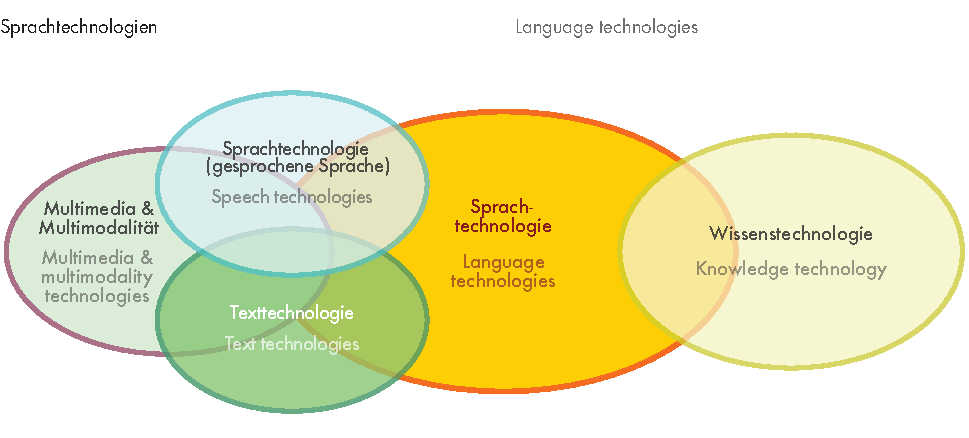
\includegraphics[width=\textwidth]{../_media/nynorsk/language_technologies}
  \caption{Språkteknologi i kontekst}
  \label{fig:ltincontext_no}
  \colorrule{grey3}{\textwidth}{1.5pt}
\end{figure*}

Når vi kommuniserer, kombinerer vi språk med andre kommunikasjonsmåtar og informasjonsmedium – til dømes kan det å snakke omfatte både gestar og andletsuttrykk. Digitale tekster kan knyte seg opp mot både bilete og lydar. Filmar kan innehalde språk i både munnleg og skriftleg form. Med andre ord er tale- og tekstteknologi overlappande, og dei samhandlar med andre teknologiske verktøy som bidreg til handsaming av multimodal kommunikasjon og multimediedokument.\\ 
I det følgjande vil vi diskutere dei viktigaste bruksområda for språkteknologi, dvs. korrekturlesing, nettsøk, taleteknologi og maskinomsetjing. Dette omfattar program og grunnleggjande teknologiar som:

\begin{itemize}
\item korrekturlesing
\item skrivestøtte
\item dataassistert språklæring
\item informasjonsinnhenting  
\item informasjonsekstrahering
\item tekstsamandrag
\item svar på spørsmål/dialogsystem
\item taleattkjenning 
\item talesyntese 
\end{itemize}

Språkteknologi er eit etablert forskingsfelt, og det finst eit omfattande utval av introduksjonslitteratur.

For vidare lesing tilrår vi lærebøkene \cite{jurafsky-martin01, manning-schuetze1}, oversiktsverka \cite{lt-survey1} og nettsida LT World (\url{http://www.lt-world.org}).

Før vi går vidare til ein diskusjon av desse bruksområda, skal vi kort skildre oppbygginga av eit typisk språkteknologisk system. 

\subsection{Applikasjonsarkitekturar}

Dataprogram for språkhandsaming består typisk av fleire komponentar som gjenspeglar ulike aspekt ved språket. Slike applikasjonar er som oftast svært komplekse, og figur~\ref{fig:textprocessingarch_no} viser ein svært forenkla arkitektur for eit vanleg teksthandsamingsprogram. Dei tre første modulane handterer strukturen og tydinga til den analyserte teksten:

\begin{enumerate}
\item Preprosessering: Reinsar data, analyserer eller fjernar formatering, identifiserer inndataspråk, osb. 
\item Grammatisk analyse: Finn verbet, identifiserer objekta til verbet, modifikatorar og andre setningskomponentar, identifiserer setningsstruktur. 
\item Semantisk analyse: Utfører disambiguering (dvs. bereknar tydinga av eit ord i ein gjeven kontekst); løyser opp anaforar (dvs. finn kva for pronomen som refererer til kva for substantiv i setninga); representerer setningstydinga på ein maskinleseleg måte.
\end{enumerate}

Etter tekstanalysen kan modular innretta mot spesifikke oppgåver takast i bruk, til dømes automatisk samandrag og databasesøk. 

I resten av denne kapitlet skal vi først gje ei skildring av dei viktigaste bruksområda for språkteknologi. Deretter følgjer eit kort oversyn over situasjonen for språkteknologisk forsking og utdanning i dag, saman med ei skildring av tidlegare og noverande forskingsprogram. Til slutt skal vi presentere eit ekspertestimat for dei viktigaste språkteknologiske verktøya og ressursane for norsk, vurdert etter ulike kriterium som tilgjenge, mogenskap og kvalitet. Den generelle situasjonen for språkteknologi for norsk språk er oppsummert i ein eigen tabell (figur~\ref{fig:lrlttable_no}), som gjev eit oppdatert oversyn over språkteknologi for norsk. Den språkteknologiske støtta for norsk språk er òg samanlikna med dei andre språka som er analyserte i denne kvitbokserien. 

\begin{figure*}[htb]
  \colorrule{grey3}{\textwidth}{1.5pt}
  \center
  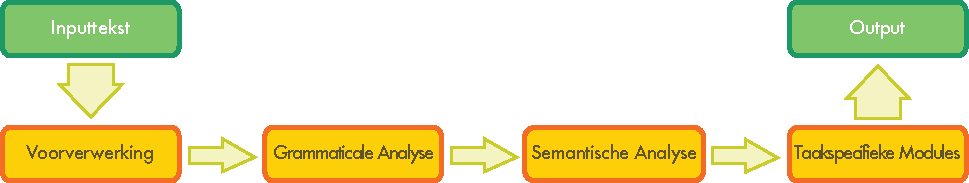
\includegraphics[width=\textwidth]{../_media/nynorsk/text_processing_app_architecture}
  \caption{Ein typisk arkitektur for tekstprosessering}
  \label{fig:textprocessingarch_no}
  \colorrule{grey3}{\textwidth}{1.5pt}
\end{figure*}

\subsection{Dei viktigaste bruksområda}

I dette avsnittet fokuserer vi på dei viktigaste språkteknologiske verktøya og ressursane, og gjev eit oversyn over språkteknologisk verksemd i Noreg.  %GIL Verktøy og ressursar som er understreka i teksten, kan også finnast i tabellen på slutten av dette kapitlet.

\subsubsection{Korrekturlesing}

Alle som har brukt eit teksthandsamingsprogram som Microsoft Word veit at det har ein stavekontroll som uthevar stavefeil og føreslår rettingar. Dei første stavekontrollane samanlikna ei liste av utvalde ord mot ei ordbok med korrekte ord. I dag er slike program langt meir sofistikerte. Ved å bruke språkspesifikke algoritmar for \textbf{grammatisk analyse} kan dei oppdage morfologiske feil (t.d. fleirtalsformer) og dessutan syntaktiske feil, til dømes manglande verb eller gal verbbøying (t.d \textit{ho *skrive eit brev}). Men dei fleste stavekontrollar vil ikkje finne nokon feil i denne engelske teksten \cite{zar1}:
 
\begin{quote}
  I have a spelling checker,\\
  It came with my PC.\\
  It plane lee marks four my revue\\
  Miss steaks aye can knot sea.
\end{quote}

For å avdekke slike feil trengst ei analyse av konteksten, til dømes for å avgjere om eit norsk ord skal stavast med enkel eller dobbel konsonant i norsk, som i \textit{vil} vs. \textit{vill}.
Denne typen analyse må anten baserast på språkspesifikke grammatikkar som ekspertar gjennom mykje arbeid har koda i programvara, eller på ein statistisk språkmodell. 
I ein statistisk modell reknar ein ut sannsynet for at eit bestemt ord finst i ein viss posisjon i teksta (t.d. mellom orda som kjem før og etter det aktuelle ordet). Til dømes er \textit{eg vil ha} ein mykje meir sannsynleg ordsekvens enn \textit{eg vill ha}. Ein statistisk språkmodell kan genererast automatisk ved hjelp av ei stor mengd av (riktige) språkdata, eit \textbf{tekstkorpus}. 

Desse to tilnærmingane har i hovudsak vorte utvikla med utgangspunkt i materiale frå engelsk. Likevel kan ingen av dei enkelt overførast til norsk, sidan norsk har annleis ordstilling, samansette ord og eit meir omfattande bøyingsmønster for visse ordklasser enn engelsk. Studiar med utgangspunkt i norsk er difor naudsynt. Sidan norsk har to offisielle målformer, der den eine er mindre brukt, er behovet for gode korrekturverktøy for kvar av målformene stort. 

\begin{figure*}[htb]
  \colorrule{grey3}{\textwidth}{1.5pt}
  \center
  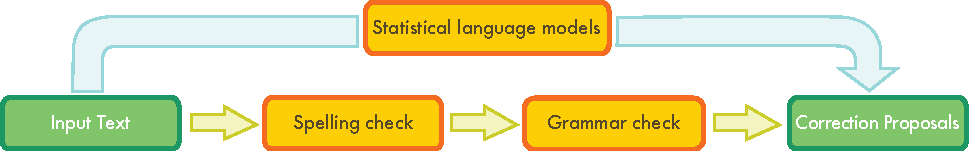
\includegraphics[width=\textwidth]{../_media/nynorsk/language_checking}
  \caption{Korrekturlesing (statistisk; regelbasert)}
  \label{fig:langcheckingaarch_no}
  \colorrule{grey3}{\textwidth}{1.5pt}
\end{figure*}

Korrekturlesingsverktøy er ikkje avgrensa til teksthandsamingsprogram, det er òg brukt i \textbf{skrivestøttesystem}, dvs. programvaresystem som blir brukte for å skrive manualar og andre typar teknisk dokumentasjon som må oppfylle spesielle standardar til dømes innan IT- og helsesektoren og innan ingeniørverksemd. I frykt for kundeklager og skadekrav som følgje av uklare instruksjonar, fokuserer næringslivet i aukande grad på teknisk dokumentasjonskvalitet, samstundes som dei rettar seg mot ein internasjonal marknad (via omsetjings- eller lokaliseringstenester). Framsteg innan prosessering av naturleg språk har ført til utvikling av programvare for skrivestøtte. Slik programvare hjelper forfattarar av teknisk dokumentasjon til å bruke ordtilfang og setningsstrukturar som er i samsvar med industrireglar og (bedriftsinterne) terminologiske restriksjonar. 

\boxtext{Korrekturlesingsverktøy blir ikkje berre brukt til teksthandsaming, det blir også brukt i skrivestøttesystem.}

Gode korrekturlesingsverktøy kan vere ein viktig reiskap for personar med skrivevanskar, anten det er dyslektikarar eller andrespråkselevar, sidan ein kontekstsensitiv analyse gjer det mogleg å føreslå færre og meir relevante stavemåtar; det motsette, mange val, krev nettopp eit høgt nivå av leseferdigheit og språkleg medvit.

Einskilde norske selskap og språktenesteleverandørar utviklar produkt på dette området. 
I forskingssektoren blir det utvikla grunnleggjande språkteknologiske ressursar som kan vere av nytte for grammatikk- og stavekontroll (leksikon, ordlister, tekstkorpus, analyseverktøy for samansette ord); desse er i hovudsak utvikla ved Universitetet i Oslo, Universitetet i Bergen og Uni Research i Bergen. 

Det mest brukte korrekturverktøyet for norsk finst i Microsoft Office-pakka, og er laga av det finske firmaet Lingsoft, medan delar av grammatikkontrollen for bokmål vart utvikla av forskarar ved Universitetet i Oslo. Stavekontroll for bokmål og nynorsk med open kjelde-teknologi som \textit{Hunspell} er også tilgjengeleg. 

Ein annan norsk kommersiell aktør er Tansa, som spesialiserer seg på korrekturverktøy tilpassa dei spesifikke behova og ordtilfanget større føretak har. 
Dei dekkjer fleire språk i tillegg til norsk bokmål og nynorsk (til dømes engelsk, tysk, spansk og fransk), og kundane spenner frå NRK til Financial Times. 
Nynodata AS tilbyr eit omsetjingsverktøy frå bokmål til nynorsk som samstundes hjelper brukaren å følgje ein konsekvent formbruk. 

Tre selskap rettar seg spesifikt mot skriftlege hjelpemiddel for dyslektikarar. To av dei, Lingit og Include, inneheld ein stavekontrollmodul i tillegg til andre lese- og skriveverktøy (ordprediksjon, tekst-til-tale-komponentar), medan MikroVerkstedet tilbyr fullføring av ord og ordprediksjon. 

Ved første augnekast synest dermed situasjonen for korrekturverktøy på norsk som god. 
Men samstundes er fleire av initiativa nokså sårbare. 
Til dømes er norsk korrekturlesing basert på open kjeldekode (\textit{aspell, Hunspell}) driven av tre einskildpersonar som gjer dette på fritida. 
Med andre ord er ein av dei viktigaste norske konkurrentane til Microsofts programvare avhengig av eit personleg initiativ frå ei handfull idealistiske einskildpersonar, snarare enn ein systematisk innsats for å utvikle modular med open kjeldekode. 
Vidare er det ei viktig utfordring for dei fleste norske korrekturlesingsverktøya å \textit{forbetre} eksisterande ressursar ved å utvikle meir avanserte språkteknologiske verktøy. Det manglar òg språkspesifikke verktøy for automatisk omsetjing og omsetjingsstøtte. Verktøy med omsetjingsminne som Trados finst, men dei har inga språkspesifikk tilpassing til norsk utover ein grunnleggjande stavekontroll. 

Utover korrekturlesnad og skrivestøtte er korrekturverktøy òg viktig innanfor dataassistert språklæring. Korrekturverktøy kan òg automatisk korrigere nettsøk, som i Google sine \textit{Meinte du…}  - forslag til korrekte nettsøk.

\subsubsection{Nettsøk}

\begin{figure*}[htb]
  \colorrule{grey3}{\textwidth}{1.5pt}
  \center
  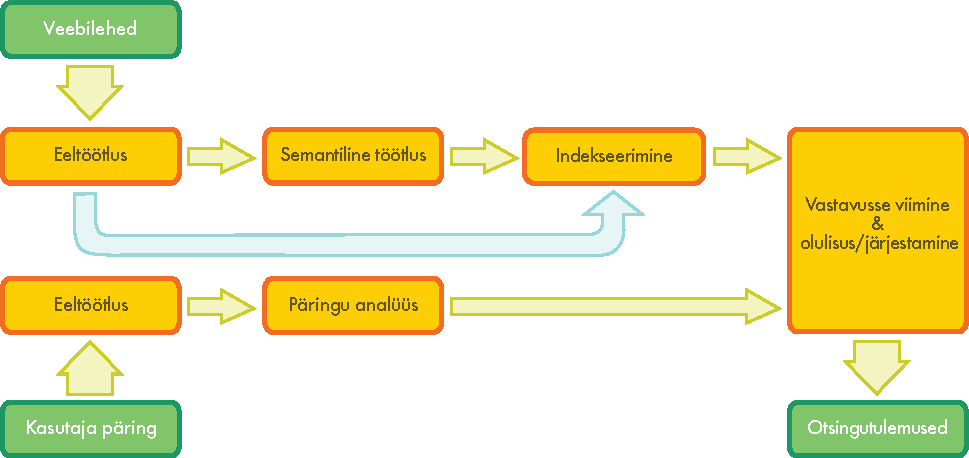
\includegraphics[width=\textwidth]{../_media/nynorsk/web_search_architecture}
  \caption{Nettsøk}
  \label{fig:websearcharch_no}
  \colorrule{grey3}{\textwidth}{1.5pt}
 \end{figure*}

Digitale søk er sannsynlegvis den mest brukte språkteknologiske applikasjonen, men han er òg i stor grad underutvikla. Søkemotoren Google, som vart oppretta i 1998, utfører no omtrent 80\% av alle nettsøk \cite{spi1}. 
Googles søkegrensesnitt og resultatvising har ikkje endra seg vesentleg sidan den første versjonen. Men i den noverande versjonen tilbyr Google stavekorrigering for feilstava ord, og har innarbeidt grunnleggjande semantiske søkemoglegheiter som kan betre nøyaktigheita gjennom analysar av tydinga til ordet i ein gjeven søkekontekst \cite{pc1}. Google sin suksess viser at med ei stor mengd tilgjengelege data kan ein statistisk orientert metode gje tilfredsstillande resultat. 

For meir sofistikerte informasjonssøk er det likevel avgjerande å integrere djupare lingvistiske analysar for teksttolking. Eksperiment med leksikalske ressursar, som maskinleselege tesaurusar eller ontologiske språkressursar (til dømes WordNet for engelsk, eit norsk ordnett er venta innan utgangen av 2012), har gjeve betre resultat når det gjeld å finne nettsider som inneheld synonym til den opphavlege søketermen, som
\textit{atomkraft}, \textit{kjerneenergi} og \textit{nukleærenergi}, og til og med termar som er endå lausare tilknytte.  

\boxtext{Den neste generasjonen søkemotorar må bruke ein mykje meir sofistikert språkteknologi.}

Den neste generasjonen søkemotorar må bruke ein mykje meir sofistikert språkteknologi, særleg for søk som består av eit spørsmål eller ein annan type setning, og ikkje berre ei liste av nøkkelord. For å svare på søket \textit{Gje meg ei liste over alle selskap som har vorte tekne over av eit anna selskap dei siste fem} må systemet gjere ein \textbf{syntaktisk} og \textbf{semantisk analyse} av setninga og lage eit hurtig oversyn over relevante dokument. Eit tilfredsstillande svar føreset ein syntaktisk analyse av den grammatiske strukturen til setninga for å slå fast at brukaren spør etter selskap som har vorte kjøpte opp, ikkje selskap som har kjøpt opp andre. Når det gjeld uttrykket \textit{dei siste fem åra}, må systemet avgjere kva for år det dreier seg om. Søket må så samanliknast mot ei stor mengd ustrukturerte data for å finne relevante treff. Dette blir kalla informasjonshenting (engelsk \textit{Information Retrieval}), og omfattar søk og rangering av relevante dokument. For å lage ei liste over selskapa treng systemet òg å forstå at ein viss ordstreng i eit dokument er namnet på eit selskap, ein prosess som blir kalla namneattkjenning. 

Ei endå større utfordring er å freiste å finne treff på eit søk i dokument på eit anna språk. Ved informasjonssøk på tvers av språk må søkeordet omsetjast automatisk til alle potensielle kjeldespråk, og resultata må deretter omsetjast tilbake til språka til brukaren. 

Sidan data i aukande grad blir oppbevart i andre format enn tekst, trengst ei teneste for multimedial informasjonsinnhenting som lèt oss søkje i bilete, lydfiler og videomateriale. Når det gjeld lyd- og videofiler, må ein taleattkjenningsmodul konvertere taleinnhaldet til tekst (eller fonetiske representasjonar) som så kan gje treff mot eit brukarsøk. 

I Noreg utvikla Opera Software den første norske nettlesaren og Internettprogramvaren. Opera byrja i 1994 som eit forskingsprosjekt i Telenor. 
Etter eit år vart det skilt ut som eit uavhengig utviklingsselskap, Opera Software ASA. Nokre norske selskap utviklar eller appliserer søkeløysingar (CognIT, Comperio, TextUrgy, Abtrox og Infofinder). 
FAST utvikla ein søkemotor som vart kjøpt opp av Microsoft, og som no blir forhandla av Comperio. 
Utviklingsfokuset til desse selskapa er hovudsakleg retta mot å tilby tilleggsprogram og avanserte søkemotorar som utnyttar domenerelevant informasjon. 
IT-industrien i Noreg har altså allereie eit ganske godt grunnlag når det gjeld nettsøk og informasjonsinnhenting; det største behovet som føretaka rapporterer om, gjeld kvalitetssikra språkteknologiske komponentar.

\subsubsection{Taleteknologi}

Dei grunnleggjande taleteknologiane er taleattkjenning og talesyntese, som kan brukast til å utvikle til dømes taleinteraksjonsteknologi og dialogsystem. Taleteknologi blir brukt for å lage grensesnitt som lèt brukarane samhandle gjennom talespråk heller enn å bruke ein grafisk skjerm, tastatur og mus. I dag blir talegrensesnitt brukt til heilt og delvis automatiserte telefontenester som selskap tilbyr kundane sine, tilsette eller partnarar. Talegrensesnitt blir brukt i stor grad til blant anna banktenester, distribusjonskjeder, kollektivtransport og i telesektoren. Taleteknologi blir òg brukt til grensesnitt for navigasjonssystem i bilar og til bruk av talespråk som eit alternativ til grafiske grensesnitt eller trykkfølsame skjermar i smarttelefonar. 

\begin{figure*}[htb]
  \colorrule{grey3}{\textwidth}{1.5pt}
  \center
  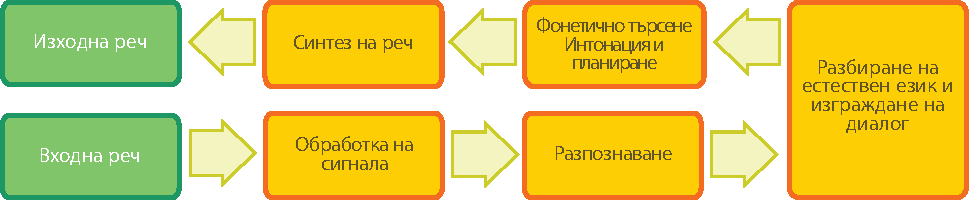
\includegraphics[width=\textwidth]{../_media/nynorsk/simple_speech-based_dialogue_architecture}
  \caption{Talebasert dialogsystem}
  \label{fig:dialoguearch_no}
  \colorrule{grey3}{\textwidth}{1.5pt}
\end{figure*}

Taleteknologi omfattar fire typar verktøy: 

\begin{enumerate}
\item Automatisk \textbf{taleattkjenning} (tale-til-tekst) avgjer orda som faktisk blir sagde i ein gjeven lydsekvens ytra av ein språkbrukar.
\item Naturleg språkforståing analyserer den syntaktiske strukturen i ytringa og tolkar ytringa ut frå systemet som blir brukt.
\item Dialogstyring avgjer kva for handling som skal utførast, gjeve ein bestemt brukarinput og ein viss systemfunksjonalitet.
\item \textbf{Talesyntese} (tekst-til-tale) omskaper svaret frå systemet til lydar som er forståelege for brukaren.
\end{enumerate}

Ei viktig utfordring for automatiske taleattkjenningssystem er å kjenne att orda som blir ytra. Det tyder at utvalet av moglege ytringar må avgrensast til eit avgrensa sett av nøkkelord, eller at ein manuelt lagar språkmodellar som dekkjer eit stort omfang av naturlege språkytringar. Ved hjelp av maskinlæringsteknikkar kan ein òg automatisk generere språkmodellar frå \textbf{talekorpus}, dvs. store samlingar av tale i lydfiler og teksttranskripsjonar. Å leggje avgrensingar på ytringane inneber vanlegvis at brukarane blir pålagde å bruke grensesnittet på ein avgrensa måte, noko som kan svekkje aksepten til brukaren av verktøyet; på den andre sida vil det auke kostnadene monaleg å skape, fininnstille og vedlikehalde rike språkmodellar. Talegrensesnitt som bruker språkmodellar og lèt brukaren uttrykkje seg meir fleksibelt i byrjinga – ved hjelp av ein førespurnad som: \textit{Kva kan eg gjere for deg?} – er generelt automatisert og gjev ofte ei betre oppleving for brukarane.

\boxtext{Taleteknologi blir brukt til å lage grensesnitt som lèt brukarane samhandle gjennom talespråk heller enn å bruke ein grafisk skjerm, tastatur og mus.}

Føretak bruker ofte førehandsinnspelt tale, innspelt av profesjonelle for å generere materialet som skal brukast i talegrensesnitt. For statiske ytringar, der formuleringane ikkje avheng av ein viss situasjon eller personlege brukardata, kan dette gje ei god brukaroppleving. Men meir dynamisk ytringsinnhald kan pregast av unaturleg intonasjonsmønster fordi dei rett og slett blir produserte ved å lime ulike lydfiler saman. Dagens talesyntese har vorte stadig betre til å produsere dynamiske ytringar som høyrest naturlege ut, sjølv om dei framleis har eit forbetringspotensial. 

Det siste tiåret har det skjedd ei betydeleg standardisering av talegrensesnitt når det gjeld dei ulike teknologiske komponentane. Det har òg vore ei sterk marknadskonsolidering innan taleteknologi. I G20-landa (dei 19 landa i verda med best økonomi og dessutan EU) har berre fem globale aktørar dominert marknaden, med Nuance (USA) og Loquendo (Italia) som dei viktigaste i Europa. I 2011 kunngjorde Nuance oppkjøpet av Loquendo, og dette innebar eit nytt steg i retning av ei sterkare konsolidering av marknaden. 

For norsk talesyntese finst tretten norske stemmer; dei fleste har vorte utvikla av aktørane vi har nemnt ovanfor. 
Tre stemmer har vorte utvikla av det norske føretaket Lingit, som rettar seg mot brukarar med lese- og skrivevanskar. 
Ei anna stemme vart utvikla ved Norsk lyd- og blindeskriftbibliotek i samarbeid med søsterbiblioteket i Sverige. 
Der er òg ei aktiv forskargruppe ved NTNU i Trondheim. 
Kvaliteten på talesyntese er sterkt avhengig av tilgjengelege ressursar (spesielt tekstkorpus tagga med informasjon om ordklasse, tokenisatorar og uttaleleksika) og språkspesifikk forsking på til dømes prosodiske trekk i det aktuelle språket. 
Det finst mange slike ressursar på engelsk, men berre i liten grad for norsk. Likevel er behovet ekstra stort for norsk på grunn av det store mangfaldet i moglege stavemåtar og dialektar, i tillegg til utfordringar knytte til tonelag og ein manglande éin-til-éin-relasjon mellom lydar og bokstavar. 

Når det gjeld teknologi og kunnskap for dialogstyring, er det norske marknaden dominert av mindre, norske føretak. 
MediaLT har utvikla ein generell taleattkjennar som blir til brukt til dialogstyring for blinde og svaksynte. 
Innan tale-til-tekst har Max Manus integrert og tilrettelagt Phillips’ SpeechMagic for norske sjukehus. 
Systemet er relativt vellukka, men har eit relativt avgrensa bruksområde med eit lukka vokabular. 
Nyleg vart Dragon Dictation, ein stemmeattkjenningsapplikasjon for mobiltelefonar, lansert for norsk. 
Denne applikasjonen er det første \textit{generelle} dikteringssystemet for norsk, men den norske versjonen av Dragon Dictation lèt til å gje betydeleg meir feiltolking enn den engelske versjonen. 
For taleinteraksjon finst det enno ikkje ein fungerande marknad for lingvistiske kjerneteknologiar for syntaktisk og semantisk analyse. 

Når ein ser framover, kan ein vente ei stor utvikling på grunn av større bruk av smarttelefonar som ei ny plattform for å handtere kunderelasjonar, i tillegg til eksisterande kommunikasjonsmedia som fasttelefonar, Internett og e-post. 
Dette vil sannsynlegvis òg påverke nytta av taleteknologi og dialogsystem. På sikt vil der sannsynlegvis bli færre telefonbaserte talegrensesnitt, og talespråksapplikasjonar vil spele ei langt meir sentral rolle som ein brukarvennleg interaksjonsmåte med smarttelefonar. 
Denne utviklinga vil sannsynlegvis primært drivast fram gjennom stegvise forbetringar av taleattkjenningssystem som ikkje er fokuserte på ein gjeven brukar, via dikteringssystem som alt blir tilbodne som sentraliserte tenester for smarttelefonbrukarar. 

\subsubsection{Maskinomsetjing}

\begin{figure*}[htb]
  \colorrule{grey3}{\textwidth}{1.5pt}
  \center
  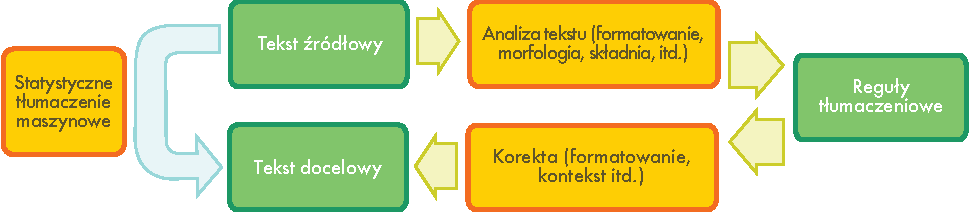
\includegraphics[width=\textwidth]{../_media/nynorsk/machine_translation}
  \caption{Maskinomsetjing (statistisk / regelbasert)}
  \label{fig:mtarch_no}
  \colorrule{grey3}{\textwidth}{1.5pt}
\end{figure*}

Tanken om å bruke datamaskiner til å omsetje naturleg språk vart introdusert i 1946, og utløyste ein omfattande forskingsinnsats på 50-talet, som så vart gjenoppliva på 80-talet. Likevel har \textbf{maskinomsetjing} (MO) framleis ikkje levd opp til dei tidlege forhåpningane om å kunne tilby generell, automatisert omsetjing.

\boxtext{Den mest grunnleggjande tilnærminga til maskinomsetjing er automatisk å erstatte ord i eitt språk med ord i eit anna språk.}

Den mest grunnleggjande tilnærminga til maskinomsetjing er automatisk å erstatte ord i eit språk med ord i eit anna språk. Dette kan fungere bra for domene der ordtilfanget er avgrensa og standardisert, som til dømes vêrmeldingar. Men for å lage gode omsetjingar av tekster frå meir generelle domene må ein omsetje større tekstbitar (ordgrupper, setningar, eller til og med heile avsnitt), og kvar tekstbit må vere i samsvar med tilsvarande del i kjeldeteksta. Maskinomsetjing er først og fremst vanskeleg fordi menneskeleg språk er fleirtydig. 

Fleirtydig språk gjev utfordringar på fleire nivå, blant anna kan ein ha bruk for å løyse det fleirtydige både på ordnivå og på setningsnivå. 
I ei enkel ord-for-ord-omsetjing til engelsk kan setninga \textit{Plutseleg rauk slangen} difor gje resultatet \textit{Suddenly smoked the snake.}
Verbforma \textit{rauk} (preteritum av \textit{ryke}) er fleirtydig mellom det vi på engelsk ville omsetje som høvesvis \textit{snap} og \textit{smoke}.
Orda \textit{slange} er på si side fleirtydig mellom `vasslange' (engelsk \textit{hose}) og `reptilslange' (engelsk \textit{snake}). Legg òg merke til at ei enkel ord-for-ord-omsetjing ikkje ville gjeve rett rekkjefølgje av orda på engelsk.

I tillegg til leksikalsk fleirtydigheit og skilnader i ordstilling kjem utfordringar med syntaktiske fleirtydigheiter. På norsk kan ein til dømes topikalisere objektet i ei setning, medan opninga for å gjere dette på engelsk er mykje meir avgrensa. Den norske setninga \textit{Epla åt mannen} har to ulike tolkingar: anten blir \textit{epla} analysert som subjektet til setninga (mannen vart eten av epla), eller som eit topikalisert objekt (epla vart etne av mannen). Sidan denne fleirtydigheita ikkje finst på engelsk, må eit maskinomsetjingssystem først finne den korrekte syntaktiske tolkinga for å kome fram til ei korrekt omsetjing.

Ei anna utfordring for maskinomsetjing for norsk er samansette ord. Eit effektivt omsetjingssystem må kunne identifisere samansette ord som ikkje står i ordboka, analysere dei, og om naudsynt lage nye samansette ord i målspråket.

For omsetjingar mellom språk som er nært i slekt kan ei enkel ord-for-ord-omsetjing la seg gjere. Men maskinomsetjingssystem kan òg byggjast ved å bruke lingvistiske reglar. Regelbaserte (eller kunnskapsdrivne) system analyserer kjeldeteksten, og lagar ein mellomståande symbolsk representasjon. På grunnlag av den symbolske representasjonen kan ein så generere tekst til målspråket. Kvaliteten på slike metodar avheng i stor grad av tilgangen til omfattande ordbøker med morfologisk, syntaktisk og semantisk informasjon, i tillegg til store sett med grammatiske reglar utvikla av språkforskarar. Dette er ein veldig omfattande, og difor dyr, prosess.

På slutten av 80-talet, då datamaskinkapasiteten auka, auka òg interessa for statistiske modellar for maskinomsetjing. Statistiske modellar for maskinomsetjing er basert på analysar av tospråklege tekstkorpus, som parallellkorpuset Europarl, som består av møtereferat frå Europaparlamentet på 11 europeiske språk 
(norsk er ikkje inkludert).
Viss ein har tilgang til tilstrekkelege mengder data, kan statistisk maskinomsetjing fungere godt nok til å finne den omtrentlege tydinga til ei tekst på eit anna språk, gjennom å prosessere parallelle versjonar av tekst og dermed finne sannsynlege ordmønster. Datadriven maskinomsetjing har sine fordelar, fordi ho krev mindre menneskeleg innsats, og kan fange opp særmerkte trekk ved språket (til dømes idiomatiske uttrykk) som kan oversjåast av kunnskapsdrivne system. Men i motsetnad til kunnskapsdrivne system gjev statistisk (eller datadrive) maskinomsetjing ofte ugrammatiske resultat.  

Ofte er det altså slik at fordelane og ulempene ved kunnskapsdriven og datadriven maskinomsetjing utfyller kvarandre. Difor fokuserer nyare forsking ofte på hybridtilnærmingar som kombinerer begge metodane. Ei slik tilnærming bruker både kunnskapsdrivne og datadrivne system saman med ein selekteringsmodul som avgjer det beste resultatet for kvar setning. For setningar lengre enn omtrent tolv ord blir likevel resultata som regel mindre gode. Her kan ei betre løysing vere å kombinere dei beste delane frå kvar setning frå fleire ulike kjelder. Dette kan vere ei ganske kompleks oppgåve, sidan det ikkje alltid er klart kva for delar som passar saman. Desse må identifiserast og parallellstillast.   

\boxtext{Sjølv om det er eit klart behov for maskinomsetjing for norsk, er utviklinga av slik programvare for norsk enno ikkje omfattande.}

Når det gjeld omsetjing mellom dei to norske målformene, er behovet for effektive omsetjingsverktøy stort. To selskap har utvikla system for dette, Nynodata og Apertium. Nynodata er eit lite føretak som tilbyr verktøy for omsetjing, korrektur og tekstsøk for bokmål og nynorsk. Apertium er eit open-kjelde-initiativ som òg tilbyr automatisert omsetjing mellom dei to målformene, implementert av ein student ved Universitetet i Bergen.

Når det gjeld omsetjing mellom norsk og ulike framandspråk, har Google Translate ein norsk modul for omsetjing mellom engelsk og norsk; via engelsk er det mogleg å omsetje mellom norsk og kvart eit språkpar som inneheld engelsk. GramTrans er ei maskinomsetjingsplattform som er utvikla av det danske GrammarSoft ApS og det norske føretaket Kaldera Språkteknologi AS. Denne omsetjingsmotoren tilbyr ei teneste for gratis, nettbasert omsetjing for dei skandinaviske språka og mellom norsk og engelsk. Programmet er basert på ein robust grammatikkanalyse, ein transferkomponent som handsamar overgangen frå eitt språk til eit anna med omsyn til leksikon og grammatikk, og til slutt ein komponent som genererer omsett tekst på målspråket. Selskapet Clue Norge spesialiserer seg på elektroniske ordbøker for næringslivet, og utvikla for omtrent ti år sidan systemet Textran for maskinomsetjing frå engelsk til norsk. Systemet eksisterer enno, men har ikkje vorte vidareutvikla fordi jamt pålitelege maskinomsetjingar av høg kvalitet er særs vanskeleg å oppnå, medan brukargruppene ikkje ynskte å betale for eit system som gjorde feil.

Sjølv om det føregår ein betydeleg forskingsinnsats på dette området, både nasjonalt og internasjonalt, har datadrivne og hybride system så langt vore mindre vellukka i applikasjonar for næringslivet enn i forskingslaboratoriet. I Noreg finst den viktigaste forskingsekspertisen ved Universitetet i Oslo og Universitetet i Bergen.

Å bruke maskinomsetjing kan auke produktiviteten betydeleg, så lenge systemet er tilpassa brukarspesifikk terminologi og er godt integrert i arbeidsflyten på ein arbeidsplass. Generelt verkar det likevel som at språktenesteindustrien i Noreg har eit underforbruk av språkteknologiske ressursar. 
Sektoren kan delast i to grupper: på den eine sida har ein frilansomsetjarar og omsetjingsbyrå som rettar seg mot einskildpersonar, næringslivet og offentleg sektor; på den andre sida har ein omsetjarar som er knytte til Oversetterforeningen og Norsk faglitterær forfatter- og oversetterforening.

I den siste gruppa verker det som språkteknologi berre er i avgrensa bruk. Den førstnemnde gruppa bruker ofte Trados, som er det klart mest brukte omsetjingsverktøyet for profesjonelle omsetjarar. Trados har likevel ingen eigen modul for norsk, men støttar seg i staden på Hunspell, ei open-kjelde-løysing med stavekontroll og eit morfologisk analyseverktøy som opphavleg vart utvikla for ungarsk. Sjølv om det er ei funksjonell og open løysing, treng ho ytterlegare utvikling for å fungere som ein optimal ressurs for språktenestesektoren i Noreg. Særleg stort er behovet for å forbetre analysen av samansette ord på norsk. 

I tillegg bruker profesjonelle omsetjarar termbasar (DU, IATE), og til ein viss grad er der eit samarbeid med universitetssektoren i utviklinga av termbasar. Det tilsynelatande underforbruket av språkteknologiske ressursar i språktenesteindustrien heng delvis saman med mangelen på gode ressursar for norsk, men òg manglande kontakt mellom språktenesteleverandørar og forskarmiljøa. Difor kan kunnskap om det fulle potensialet for språkteknologi bli for avgrensa, og det kan vere vanskeleg for kommersielle aktørar å vurdere kvaliteten på eksisterande ressursar.

Kvaliteten på maskinomsetjingssystem har framleis eit stort forbetringspotensial. Blant utfordringane er å tilpasse språkressursar til eit gjeve emne eller brukarområde, og å integrere teknologien i ein arbeidsflyt som alt inneheld termbasar og omsetjingsminne. I tillegg er dei fleste systema som er i bruk retta mot engelsk, og støttar berre sjeldan omsetjing til og frå norsk. Dette gjev forstyrringar i prosessen med å få tekst omsett, og tvingar maskinomsetjingsbrukarar til å lære seg ulike kodingsverktøy for ulike system.

Gjennom evalueringskampanjar samanliknar forskarar kvaliteten på ulike maskinomsetjingssystem og tilnærmingar og ikkje minst kva som er status for systema for ulike språkpar.
Prosjektet EuroMatrixPlus gjennomførde ein studie av kvaliteten på maskinomsetjingssystem for 22 offisielle EU-språk.
Norsk var ikkje inkludert i dette prosjektet.

\subsection{Andre bruksområde}

Oppbygginga av språkteknologiske verktøy omfattar ei rekkje underoppgåver som ikkje alltid er synlege på overflata, der kommunikasjonen med brukaren skjer. Slike underliggjande program har likevel viktige funksjonar i systemet. Kvar av oppgåvene utgjer viktige forskingsfelt, som har utvikla seg til enkeltdisiplinar innanfor datalingvistikk.

Såkalla dialogsystem som svarer på spørsmål (engelsk \textit{Question Answering}) er til dømes eit aktivt forskingsområde, der ein har utvikla korpus koda med setningsstruktur, og der vitskaplege evalueringskonkurransar har vore initierte. Feltet omfattar meir enn berre søk på nøkkelord (der søkemotoren svarar med ei samling potensielt relevante dokument); det lèt brukarar stille konkrete spørsmål som systemet så gjev eitt einaste svar på. Til dømes:

\begin{quote}
Spørsmål: \textit{Kor gammal var Neil Armstrong då han gjekk på månen?}\\
Svar: \textit{38.}
\end{quote}

Medan slike dialogsystem openbert er relaterte til nettsøk, blir det i dag nytta som eit overordna omgrep for forskingsspørsmål som kva for typar spørsmål som finst, korleis ein skal handsame dei, korleis ein kan analysere og samanlikne sett av dokument som potensielt inneheld svaret (gjev dokumenta til dømes motstridande svar?), og korleis relevant informasjon kan ekstraherast frå eit dokument med minimal grad av feil, og utan å sjå bort frå kontekst.

Dette er i sin tur knytt til informasjonsekstrahering (engelsk \textit{Information Extraction}), eit område som vart svært populært og innflytelsesrikt då datalingvistikken fekk ei meir statistisk orientering tidleg på 90-talet. Informasjonsekstrahering har som mål å finne bestemte bitar av informasjon i visse sett av dokument, til dømes å identifisere dei viktigaste aktørane i avisartiklar som handlar om å ta over føretak. Eit anna scenario som kan studerast, er terrorhandlingar. Problemstillinga er då å sortere informasjon i teksten i samsvar med ein førehandsdefinert mal som spesifiserer kriterium som gjerningsmann, mål, tid, stad og utfall av hendinga. Informasjonsekstrahering består grunnleggjande sett i å fylle ut ein mal med domenespesifikk og relevant informasjon, noko som gjer informasjonsekstrahering til nok eit døme på ein underliggjande teknologi som på den eine sida utgjer eit sjølvstendig forskingsfelt, og som på den andre sida skal kunne integrerast i større brukarapplikasjonar for praktisk nytte.

\textbf{Samandrag} og \textbf{tekstgenerering} er tilgrensande område som kan brukast som sjølvstendige applikasjonar eller som underliggjande støtteteknologi. Samandrag har som mål å gje att dei viktigaste punkta i ei lengre tekst, og finst blant anna i Microsoft Word. Oftast blir det brukt ei statistisk tilnærming for å identifisere dei `viktige' orda i ei tekst (dvs. ord som opptrer hyppig i den aktuelle teksta, men meir sjeldan i allmennspråket) og for å finne dei setningane som har høgast førekomst av desse `viktige' orda. Dei aktuelle setningane blir så trekte ut og sette saman for å lage eit samandrag. I ein slik modell, som er svært utbreidd i kommersiell nytte, er samandrag rett og slett ei form for ekstrahering av setningar, og teksta blir redusert til eit subsett av setningane sine. Eit anna alternativ er å generere heilt nye setningar som ikkje allereie finst i kjeldeteksten, og ein del forsking blir gjort på dette feltet.

\boxtext{Forsking på dei fleste typar tekstteknologi er langt mindre utvikla for norsk enn for engelsk.}

Å generere nye setningar som oppsummerer originaltekst krev ei djupare forståing av teksta, og denne tilnærminga er difor så langt betydeleg mindre robust. Generelt blir ein tekstgenerator sjeldan brukt som ein sjølvstendig applikasjon, men blir i staden integrert i eit større programvaremiljø, som til dømes eit informasjonssystem om kliniske data som samlar, lagrar og prosesserer pasientopplysningar. Rapportgenerering er berre eitt av mange potensielle bruksområde for samandrag.
I USA har det sidan 90-talet vore fleire opne konkurransar i å svare på spørsmål automatisk eller dialogsystem, informasjonsekstrahering og samandrag, som først og fremst har vore arrangert av dei offentlege støtta organisasjonane DARPA og NIST. Gjennom desse konkurransane har teknologien vorte klart forbetra, men hovudfokus har altså vore på engelsk. 
Det finst nesten ikkje annoterte korpus eller andre spesialressursar for å utføre slike oppgåver på norsk. 
Når tekstoppsummeringssystem utelukkande bruker statistiske metodar, er dei i høg grad språkuavhengige, og det finst mange tilgjengelege forskingsprototypar. 
For tekstgenerering har komponentar som kan brukast om att stort sett vore avgrensa til modular for produksjon av overflatestrukturen, og det meste av tilgjengeleg programvare er for engelsk. 

\subsection{Utdanningsprogram}

Språkteknologi er eit interdisiplinært fagfelt som samlar ekspertise frå bl.a. språkforsking, informatikk, matematikk, filosofi, psykolingvistikk og nevrovitskap.
Difor har ikkje språkteknologi fått etablert ein klart definert, sjølvstendig plass i det norske universitetssystemet. 

I Noreg finst den språkvitskaplege ekspertisen i mindre forskargrupper ved ulike institusjonar som samarbeider på prosjektbasis (Universiteta i Oslo, Bergen og Tromsø, NTNU, NHH og forskingsinstitusjonane Uni Research og Sintef). Ingen av universiteta har eigne institutt eller senter for datalingvistikk. Undervising i datalingvistikk føregår anten ved institutt for informatikk (Universitetet i Oslo og NTNU) eller lingvistikk (Universiteta i Bergen og Tromsø). Forsking og undervising i taleprosessering føregår berre ved NTNU.

Sjølv om det er vanskeleg å kvantifisere ein slik påstand, er det nok rimeleg å hevde at datalingvistikk og språkteknologi, så vel som høva for å studere dette i Noreg, ikkje er særleg godt kjend i Noreg. Eit viktig mål for KUNSTI-programmet var å styrkje grunnforsking og kompetansen innanfor dei språkteknologiske fagfelta. KUNSTI bidrog til fleire masteroppgåver og doktoravhandlingar innanfor ei rekkje forskingsprosjekt. Forskingsprogrammet spelte dermed ei viktig rolle for å skaffe norsk språkteknologi nye forskarar og auka kompetanse.

Universitetet i Bergen koordinerer CLARA, eit nettverk for forskarutdanning innan SRT ved ni europeiske institusjonar.

\subsection{Nasjonale prosjekt og initiativ}

Sidan norsk språkteknologisk industri er relativt liten i internasjonal samanheng, har norske forskingsinstitusjonar spelt ei sentral rolle i utviklinga av norske ressursar og verktøy for språkteknologi, noko som òg har kome private føretak til nytte. 
Dei fleste norske selskap som treng språkteknologi, uttrykkjer eit ynske om å kunne nyttiggjere seg ressursar, kunnskap og ekspertise frå akademia, fordi deira eigen ekspertise vanlegvis ikkje ligg innanfor språkteknologi. 

Noregs forskingsråd har så langt støtta eitt betydeleg språkteknologisk forskingsprogram, nemleg KUNSTI (Kunnskapsutvikling for norsk språkteknologi). 
Dette programmet var delvis inspirert av større prosjekt i andre land (til dømes det tyske prosjektet Verbmobil), og hadde som mål å auke kompetansen om språkteknologi gjennom grunnforsking. KUNSTI skulle gjere skriftleg og munnleg norsk (og til ein viss grad samisk) tilgjengeleg for databehandling gjennom forsking og utvikling. Tjue forskingsprosjekt av ulike storleikar vart gjennomførde i løpet av programperioden; dei to største var innan maskinomsetjing og taleteknologi.

Å byggje opp eit mangfald av språkteknologiske applikasjonar føreset tilgjenge på grunnleggjande ressursar, som ordlister, tekstkorpus og talekorpus. Slike ressursar er like dyre og tidkrevjande å utvikle for små språk som for store; sidan norsk har to offisielle målformer blir kostnadene endå høgare. 
Difor er ikkje norsk så interessant frå ein kommersiell ståstad.

Difor var det eit viktig språkpolitisk tiltak at Språkbanken vart oppretta i 2010, etter tjue år med felles innsats frå Språkrådet, Noregs forskingsråd, næringslivet og norske forskingsinstitusjonar. Språkbanken ved Nasjonalbiblioteket skal fungere som ein infrastruktur for å gjere norsk språkteknologi tilgjengeleg både for forsking og kommersiell utvikling, noko som vonleg vil senke terskelen for å utvikle nye språkteknologiske produkt for norsk. 

Så langt har private selskap typisk bygd ulike ressursar og verktøy til intern bruk, medan dei fleste omfattande (og tilgjengelege) ressursar og verktøy (til dømes leksikon, taggarar og namneattkjennarar) er utvikla ved forskingsinstitusjonane. På eit seinare tidspunkt har desse ressursane i nokre tilfelle vorte kjøpte av private føretak. Faktisk inneheld tabellen over verktøy og ressursar i slutten av denne rapporten hovudsakleg ressursar som er utvikla gjennom forsking. Til dømes har Universitetet i Oslo utvikla talekorpuset Nota-Oslo (Norsk Talespråkskorpus, Oslo-delen) og Nordisk dialektkorpus, Norsk ordbank er utvikla og er ått av Universitetet i Oslo og Norsk språkråd, Oslo-Bergen-taggaren er laga av Universitetet i Oslo og Uni Research i Bergen, Norsk aviskorpus er utvikla av Uni Research og NHH, og trebanken INESS blir for tida bygd opp ved Universitetet i Bergen.

Utvikling av grunnleggjande tekst- og taledata var ikkje ein del av Kunstis arbeidsprogram, sidan dette skulle vere ei oppgåve for Språkbanken. Mangelen på grunnleggjande språkressursar stod dermed fram som ein hemsko for KUNSTI. No som Språkbanken er etablert, og med nye forskarar og oppdatert kompetanse på plass, meiner mange at tida er moden for ei ny satsing på språkteknologisk forsking som kan få eit meir applikasjonsorientert fokus enn KUNSTI-satsinga.

Etter KUNSTI har større språkteknologiske forskingsprosjekt (til dømes INESS, Nota-Oslo (Norsk Talespråkskorpus, Oslo-delen), Norsk aviskorpus, WeSearch-Språkteknologi for internett og SIRKUS) vorte finansierte anten gjennom infrastrukturprogramma (AVIT) eller forskingsrådets generelle IKT-program, som VERDIKT. 
Som eit ledd i arbeidet med å byggje opp ein norsk infrastruktur for språkressursar inngjekk Språkbanken i 2011 ein avtale med Kaldera språkteknologi AS om å byggje eit ordnett for bokmål og nynorsk. Trass i desse investeringane er likevel støtta til språkteknologiske prosjekt i Noreg relativt låg samanlikna med det som blir brukt til dømes i USA på omsetjing og fleirspråkleg informasjonstilgang \cite{laz1}.

Som ei oppsummering har dette delkapitlet vist at tidlegare forskingsprogram har ført til ei utvikling av ei rekkje språkteknologiske verktøy og ressursar for norsk språk. 
I neste delkapittel oppsummerer vi situasjonen for språkteknologisk støtte for norsk språk. 

\subsection{Situasjonen for språkteknologisk støtte for norsk språk}
Figur~\ref{fig:lrlttable_no} oppsummerer situasjonen for språkteknologisk støtte for norsk språk gjennom talvurderingar av eksisterande verktøy og ressursar. Vurderingane er gjorde av leiande norske ekspertar på feltet, som har sett talverdiar for sju ulike kriterium (t.d. tilgjenge), på ein skala frå 0 (svært låg) til 6 (svært høg).

%Numbers have been inserted, but it would be good to go over them
\begin{figure*}[htb]
\centering
%\begin{tabular}{>{\columncolor{orange1}}p{.33\linewidth}ccccccc} % ORIGINAL
\begin{tabular}{>{\columncolor{orange1}}p{.33\linewidth}@{\hspace{6mm}}c@{\hspace{6mm}}c@{\hspace{6mm}}c@{\hspace{6mm}}c@{\hspace{6mm}}c@{\hspace{6mm}}c@{\hspace{6mm}}c}
\rowcolor{orange1}
 \cellcolor{white}&\begin{sideways}\makecell[l]{Kvantitet}\end{sideways}
&\begin{sideways}\makecell[l]{\makecell[l]{Tilgjengelegheit} }\end{sideways} &\begin{sideways}\makecell[l]{Kvalitet}\end{sideways}
&\begin{sideways}\makecell[l]{Dekningsgrad}\end{sideways} &\begin{sideways}\makecell[l]{Modenheit}\end{sideways} &\begin{sideways}\makecell[l]{Berekraft}\end{sideways} &\begin{sideways}\makecell[l]{Tilpassingsdyktigheit}\end{sideways} \\ \addlinespace
\multicolumn{8}{>{\columncolor{orange2}}l}{Språkteknologi (verktøy, teknologiar og applikasjonar)} \\ \addlinespace
Taleattkjenning &4&2&2&1&2&3&3 \\ \addlinespace
Talesyntese &3&2&3&2&3&3&3\\ \addlinespace
Setningsanalyse &4&4,5&4&4&4,5&4,5&5\\ \addlinespace
Teksttolking &2&2&3,3&3&3,7&3,3&3,7\\ \addlinespace
Språkgenerering &1&4&4&3&5&4&5\\ \addlinespace
Maskinomsetjing &4&4&2&2&3&5&3\\ \addlinespace
\multicolumn{8}{>{\columncolor{orange2}}l}{Språkressursar (ressurs-, data- og kunnskapsbasar)} \\ \addlinespace
Tekstkorpus &4,5&3,5&3,5&3&4&4,5&4\\ \addlinespace
Talekorpus &5&4&3&5&4&5&5\\ \addlinespace
Parallellkorpus &5&3&2&2&4&3&3\\ \addlinespace
Leksikalske ressursar &2,5&2&2&2&2&2&2,5\\ \addlinespace
Grammatikkar &2&4&5&3&4&5&3\\
\end{tabular}
\caption{Status for SRT for norsk}
\label{fig:lrlttable_no}
\end{figure*}

Dei viktigaste resultata for norsk kan oppsummerast slik: 

\begin{itemize}
\item Situasjonen for norsk er relativt god når det gjeld dei mest grunnleggjande språkteknologiske verktøya og ressursane, som taggarar, morfologisk analyse, referansekorpus og talekorpus.
Det finst òg mange talesynteseprodukt for norsk som er generelt brukande og som har ein akseptabel kvalitet, sjølv om dei fleste av dei er utvikla av kommersielle aktørar, og dermed har avgrensa tilgjenge. Der finst fleire leksikalske ressursar som dekkjer allmennspråket, men der er betydelege manglar når det gjeld terminologi for spesialiserte domene.
\item Det finst òg ressursar og verktøy med avgrensa funksjonalitet innan felt som taleattkjenning, maskinomsetjing og teksttolking. Nokre av desse områda blir likevel dekte hovudsakleg av kommersielle aktørar, og har dermed avgrensa tilgjenge.
\item For enkelte typar verktøy og ressursar finst nesten ingen ressursar, medan andre ressursar er utvikla for kommersielle føremål og er ikkje allment tilgjengelege. 
Dette gjeld til dømes verktøy og ressursar for meir avansert språkteknologi for norsk, som avansert diskursprosessering, tekstgenerering og ontologiar som representerer verdskunnskap.
\item Mange verktøy og ressursar manglar standardisering, det vil seie at sjølv om dei eksisterer, er dei ikkje nødvendigvis i standardformat som sikrar at dei er, og blir verande, brukande og enkle å tilpasse nye bruksområde.
Sjølv om tabellen viser at grunnleggjande verktøy og ressursar finst for norsk, er dei i nokre tilfelle fragmenterte, og nytteverdien er avgrensa av restriksjonar på bruk, inkompatibilitet med andre system og manglande dokumentasjon. 
\end{itemize}

Kort oppsummert har vi i dag tilgjengelege ressursar og verktøy med avgrensa funksjonalitet på ei rekkje felt for norsk språkteknologi.
Det er heilt tydeleg naudsynt med ei ytterlegare satsing for å rette opp dei noverande manglane med omsyn til djupare semantisk prosessering av språk og for å produsere fleire ressursar, som parallelle korpus for maskinomsetjing.

\subsection{Samanlikning på tvers av språk}

\begin{figure*}[tb]
  \small
  \centering
  \begin{tabular}
  { % defines color for each column.
  >{\columncolor{corange5}}p{.13\linewidth}@{\hspace{.040\linewidth}}
  >{\columncolor{corange4}}p{.13\linewidth}@{\hspace{.040\linewidth}}
  >{\columncolor{corange3}}p{.13\linewidth}@{\hspace{.040\linewidth}}
  >{\columncolor{corange2}}p{.13\linewidth}@{\hspace{.040\linewidth}}
  >{\columncolor{corange1}}p{.13\linewidth} 
  }
  \multicolumn{1}{>{\columncolor{white}}c@{\hspace{.040\linewidth}}}{\textbf{Framifrå}} & 
  \multicolumn{1}{@{}>{\columncolor{white}}c@{\hspace{.040\linewidth}}}{\textbf{God}} &
  \multicolumn{1}{@{}>{\columncolor{white}}c@{\hspace{.040\linewidth}}}{\textbf{Middels god}} &
  \multicolumn{1}{@{}>{\columncolor{white}}c@{\hspace{.040\linewidth}}}{\textbf{Fragmentarisk}} &
  \multicolumn{1}{@{}>{\columncolor{white}}c}{\textbf{Låg eller inga}} \\ 
  \multicolumn{1}{>{\columncolor{white}}c@{\hspace{.040\linewidth}}}{\textbf{støtte}} & 
  \multicolumn{1}{@{}>{\columncolor{white}}c@{\hspace{.040\linewidth}}}{\textbf{støtte}} &
  \multicolumn{1}{@{}>{\columncolor{white}}c@{\hspace{.040\linewidth}}}{\textbf{støtte}} &
  \multicolumn{1}{@{}>{\columncolor{white}}c@{\hspace{.040\linewidth}}}{\textbf{støtte}} &
  \multicolumn{1}{@{}>{\columncolor{white}}c}{\textbf{støtte}} \\ \addlinespace
  
& \vspace{0.5mm}engelsk
& \vspace{0.5mm}
finsk \newline 
fransk \newline 
italiensk \newline  
nederlandsk \newline 
portugisisk \newline 
spansk \newline
tsjekkisk \newline 
tysk \newline   
& \vspace{0.5mm}baskisk \newline 
bulgarsk \newline 
dansk \newline 
estisk \newline 
galisisk\newline 
gresk \newline  
irsk \newline  
katalansk \newline 
norsk \newline 
polsk \newline 
serbisk \newline 
slovakisk \newline 
slovensk \newline 
svensk \newline
ungarsk  \newline
& \vspace{0.5mm}
islandsk \newline  
kroatisk \newline 
latvisk \newline 
litausk \newline 
maltesisk \newline 
rumensk\\
\end{tabular}
\caption{Taleprosessering: status for språkteknologistøtte for 30 europeiske språk}
\label{fig:speech_cluster_no}
\end{figure*}

\begin{figure*}[tb]
  \small
  \centering
  \begin{tabular}
  { % defines color for each column.
  >{\columncolor{corange5}}p{.13\linewidth}@{\hspace{.040\linewidth}}
  >{\columncolor{corange4}}p{.13\linewidth}@{\hspace{.040\linewidth}}
  >{\columncolor{corange3}}p{.13\linewidth}@{\hspace{.040\linewidth}}
  >{\columncolor{corange2}}p{.13\linewidth}@{\hspace{.040\linewidth}}
  >{\columncolor{corange1}}p{.13\linewidth} 
  }
  \multicolumn{1}{>{\columncolor{white}}c@{\hspace{.040\linewidth}}}{\textbf{Framifrå}} & 
  \multicolumn{1}{@{}>{\columncolor{white}}c@{\hspace{.040\linewidth}}}{\textbf{God}} &
  \multicolumn{1}{@{}>{\columncolor{white}}c@{\hspace{.040\linewidth}}}{\textbf{Middels god}} &
  \multicolumn{1}{@{}>{\columncolor{white}}c@{\hspace{.040\linewidth}}}{\textbf{Fragmentarisk}} &
  \multicolumn{1}{@{}>{\columncolor{white}}c}{\textbf{Låg eller inga}} \\ 
  \multicolumn{1}{>{\columncolor{white}}c@{\hspace{.040\linewidth}}}{\textbf{støtte}} & 
  \multicolumn{1}{@{}>{\columncolor{white}}c@{\hspace{.040\linewidth}}}{\textbf{støtte}} &
  \multicolumn{1}{@{}>{\columncolor{white}}c@{\hspace{.040\linewidth}}}{\textbf{støtte}} &
  \multicolumn{1}{@{}>{\columncolor{white}}c@{\hspace{.040\linewidth}}}{\textbf{støtte}} &
  \multicolumn{1}{@{}>{\columncolor{white}}c}{\textbf{støtte}} \\ \addlinespace
  
& \vspace{0.5mm} engelsk 
& \vspace{0.5mm} 
fransk \newline 
spansk
& \vspace{0.5mm}
italiensk \newline 
katalansk \newline 
nederlandsk \newline 
polsk \newline 
rumensk \newline 
tysk \newline 
ungarsk \newline
& \vspace{0.5mm}baskisk \newline 
bulgarsk \newline 
dansk \newline 
estisk \newline 
finsk \newline 
galisisk \newline 
gresk \newline 
irsk \newline 
islandsk \newline 
kroatisk \newline 
latvisk \newline 
litausk \newline 
maltesisk \newline 
norsk \newline 
portugisisk \newline 
serbisk \newline 
slovakisk \newline 
slovensk \newline 
svensk \newline 
tsjekkisk \newline
\end{tabular}
\caption{Maskinomsetjing: status for språkteknologistøtte for 30 europeiske språk}
\label{fig:mt_cluster_no}
\end{figure*}

\begin{figure*}[tb]
  \small
  \centering
  \begin{tabular}
  { % defines color for each column.
  >{\columncolor{corange5}}p{.13\linewidth}@{\hspace{.040\linewidth}}
  >{\columncolor{corange4}}p{.13\linewidth}@{\hspace{.040\linewidth}}
  >{\columncolor{corange3}}p{.13\linewidth}@{\hspace{.040\linewidth}}
  >{\columncolor{corange2}}p{.13\linewidth}@{\hspace{.040\linewidth}}
  >{\columncolor{corange1}}p{.13\linewidth} 
  }
  \multicolumn{1}{>{\columncolor{white}}c@{\hspace{.040\linewidth}}}{\textbf{Framifrå}} & 
  \multicolumn{1}{@{}>{\columncolor{white}}c@{\hspace{.040\linewidth}}}{\textbf{God}} &
  \multicolumn{1}{@{}>{\columncolor{white}}c@{\hspace{.040\linewidth}}}{\textbf{Middels god}} &
  \multicolumn{1}{@{}>{\columncolor{white}}c@{\hspace{.040\linewidth}}}{\textbf{Fragmentarisk}} &
  \multicolumn{1}{@{}>{\columncolor{white}}c}{\textbf{Låg eller inga}} \\ 
  \multicolumn{1}{>{\columncolor{white}}c@{\hspace{.040\linewidth}}}{\textbf{støtte}} & 
  \multicolumn{1}{@{}>{\columncolor{white}}c@{\hspace{.040\linewidth}}}{\textbf{støtte}} &
  \multicolumn{1}{@{}>{\columncolor{white}}c@{\hspace{.040\linewidth}}}{\textbf{støtte}} &
  \multicolumn{1}{@{}>{\columncolor{white}}c@{\hspace{.040\linewidth}}}{\textbf{støtte}} &
  \multicolumn{1}{@{}>{\columncolor{white}}c}{\textbf{støtte}} \\ \addlinespace

& \vspace{0.5mm}engelsk
& \vspace{0.5mm}
  fransk \newline 
  italiensk \newline 
  nederlandsk \newline 
  spansk
  tysk \newline 
& \vspace{0.5mm}baskisk \newline 
  bulgarsk \newline 
  dansk \newline 
  finsk \newline 
  galisisk \newline 
  gresk \newline 
  katalansk \newline 
  norsk \newline 
  polsk \newline 
  portugisisk \newline 
  rumensk \newline 
  slovakisk \newline 
  slovensk \newline 
  svensk \newline 
  tsjekkisk \newline 
  ungarsk \newline 
& \vspace{0.5mm}
  estisk \newline 
  irsk \newline 
  islandsk \newline 
  kroatisk \newline 
  latvisk \newline 
  litausk \newline 
  maltesisk \newline 
  serbisk \\
  \end{tabular}
\caption{Tekstanalyse: status for språkteknologistøtte for 30 europeiske språk}
\label{fig:text_cluster_no}
\end{figure*}

\begin{figure*}[tb]
  \small
  \centering
  \begin{tabular}
  { % defines color for each column.
  >{\columncolor{corange5}}p{.13\linewidth}@{\hspace{.040\linewidth}}
  >{\columncolor{corange4}}p{.13\linewidth}@{\hspace{.040\linewidth}}
  >{\columncolor{corange3}}p{.13\linewidth}@{\hspace{.040\linewidth}}
  >{\columncolor{corange2}}p{.13\linewidth}@{\hspace{.040\linewidth}}
  >{\columncolor{corange1}}p{.13\linewidth} 
  }
  \multicolumn{1}{>{\columncolor{white}}c@{\hspace{.040\linewidth}}}{\textbf{Framifrå}} & 
  \multicolumn{1}{@{}>{\columncolor{white}}c@{\hspace{.040\linewidth}}}{\textbf{God}} &
  \multicolumn{1}{@{}>{\columncolor{white}}c@{\hspace{.040\linewidth}}}{\textbf{Middels god}} &
  \multicolumn{1}{@{}>{\columncolor{white}}c@{\hspace{.040\linewidth}}}{\textbf{Fragmentarisk}} &
  \multicolumn{1}{@{}>{\columncolor{white}}c}{\textbf{Låg eller inga}} \\ 
  \multicolumn{1}{>{\columncolor{white}}c@{\hspace{.040\linewidth}}}{\textbf{støtte}} & 
  \multicolumn{1}{@{}>{\columncolor{white}}c@{\hspace{.040\linewidth}}}{\textbf{støtte}} &
  \multicolumn{1}{@{}>{\columncolor{white}}c@{\hspace{.040\linewidth}}}{\textbf{støtte}} &
  \multicolumn{1}{@{}>{\columncolor{white}}c@{\hspace{.040\linewidth}}}{\textbf{støtte}} &
  \multicolumn{1}{@{}>{\columncolor{white}}c}{\textbf{støtte}} \\ \addlinespace
    
& \vspace{0.5mm}engelsk
& \vspace{0.5mm} 
    fransk \newline 
    italiensk \newline
    nederlandsk \newline 
    polsk \newline
    spansk \newline
    svensk \newline 
    tsjekkisk \newline 
    tysk \newline 
    ungarsk \newline
& \vspace{0.5mm} baskisk\newline 
    bulgarsk \newline 
    dansk \newline 
    estisk \newline 
    finsk \newline 
    galisisk \newline 
    gresk \newline 
    katalansk \newline 
    kroatisk \newline 
    norsk \newline 
    portugisisk \newline 
    rumensk \newline 
    serbisk \newline 
    slovakisk \newline 
    slovensk \newline
&  \vspace{0.5mm}
    irsk \newline 
    islandsk \newline 
    latvisk \newline 
    litausk \newline 
    maltesisk  \\
  \end{tabular}
  \caption{Tale- og tekstressursar: status for språkteknologistøtte for 30 europeiske språk}  
  \label{fig:resources_cluster_no}
\end{figure*}

Situasjonen for språkteknologi varierer mykje frå språk til språk. For å samanlikne situasjonen for ulike språk presenterer vi i dette delkapitlet ei vurdering basert på to utvalde applikasjonsområde (maskinomsetjing og taleprosessering), ein underliggjande teknologi (tekstanalyse), og grunnleggjande ressursar som trengst for å byggje språkteknologiske applikasjonar. Språka vart delte inn på ein skala med fem kategoriar:

\begin{enumerate}
\item Framifrå støtte
\item God støtte
\item Middels god støtte 
\item Fragmentarisk støtte
\item Låg eller inga støtte
\end{enumerate}

Den språkteknologiske støtta vart målt ut frå følgjande kriterium:

\textbf{Taleprosessering:} Kvaliteten til eksisterande taleattkjenning, kvaliteten til eksisterande talesyntese, dekning av ulike domene, mengda og omfanget av eksisterande talekorpus, mengda og spreiinga av tilgjengelege talebaserte applikasjonar.

\textbf{Maskinomsetjing:} Kvaliteten til eksisterande omsetjingsteknologiar, mengda språkpar, dekninga for språklege konstruksjonar og domene, og kvaliteten til, og omfanget av, tilgjengelege system.

\textbf{Tekstanalyse:} Kvaliteten til, og dekningsgraden av, eksisterande teknologiar for tekstanalyse (morfologisk, syntaktisk, semantisk), dekninga av språklege konstruksjonar og domene, mengda og omfanget av eksisterande (annoterte) korpus, kvaliteten og dekningsgraden for eksisterande leksikalske ressursar (t.d. ordnett) og grammatikkar.

\textbf{Ressursar:} Kvaliteten og omfanget av eksisterande tekstkorpus, talekorpus og parallelle korpus, kvaliteten og dekningsgraden for eksisterande leksikalske ressursar og grammatikkar.

Figurane~\ref{fig:speech_cluster_no} til~\ref{fig:resources_cluster_no} viser tydeleg at språkteknologiske ressursar og verktøy for norsk enno ikkje har same kvalitet og dekningsgrad som ressursar og verktøy ein kan samanlikne med for engelsk. Men sjølv for dette språket som ligg på toppen, er det enno manglar når det gjeld høgkvalitetsapplikasjonar. 
Den norske situasjonen er godt i samsvar med nabolanda, sjølv om tala ikkje viser skilnadene som finst mellom bokmål og nynorsk.

Fleire norsktalande stemmer for talesyntese er tilgjengelege i ulike sluttbrukarapplikasjonar, men dei vanlege operativsystema tilbyr ikkje norsk talesyntese som kan brukast av utviklarar. 
For taleattkjenning er det lita støtte for norsk, og det finst ingen generelle taleattkjennarar, med eit mogleg unntak av Dragon Dictation, ein ny mobilapplikasjon som ikkje var tilgjengeleg i tide til å bli vurdert i denne rapporten.
Det finst eitt spesialisert dikteringsverktøy for helsevesenet med varierande kvalitet.

For maskinomsetjing mellom norsk bokmål og nynorsk finst det eitt tovegs, fritt tilgjengeleg program og eitt einvegs, kommersielt program. 
For maskinomsetjing mellom norsk og andre språk finst det eitt gratis, fritt tilgjengeleg program og eitt kommersielt program. Begge har varierande kvalitet og yting.

Komponentar for tekstanalyse dekkjer det norske språket til ein viss grad, og inngår i fleire applikasjonar som typisk gjennomfører ein nokså overflatisk språkanalyse, t.d. generelle stavekontrollar eller skrivestøtte for dyslektikarar.

Med omsyn til ressursar har vi alt tidlegare peikt på manglar.
For å byggje meir avanserte program, til dømes maskinomsetjing, er det eit tydeleg behov for ressursar og verktøy som dekkjer eit breiare utval av språklege fenomen samt utfører ein djupare semantisk analyse. Betre kvalitet og dekningsgrad vil kunne takle eit breitt spekter av avanserte bruksområde, blant anna generell maskinomsetjing av høg kvalitet.

\subsection{Oppsummering}

\emph{Denne kvitebokserien er meint som eit viktig første tiltak for å vurdere situasjonen for språkteknologi for 30 europeiske språk, og å gje ei overordna samanlikning på tvers av språka. Gjennom denne analysen av manglar og behov er det europeiske språkteknologimiljøet og andre interesserte no i stand til å utvikle eit forskings- og utviklingsprogram i stor skala, der målet er å byggje eit verkeleg fleirspråkleg Europa basert på moderne språkteknologi.}

Vi har sett at det er store skilnader frå språk til språk. Medan det finst programvare og ressursar av høg kvalitet for enkelte språk og bruksområde, er det betydelege manglar for andre (vanlegvis `mindre') språk og bruksområde. Mange språk manglar grunnleggjande verktøy for tekstanalyse og grunnlagsressursane som trengst for å utvikle dei. Andre språk har grunnleggjande verktøy og ressursar, men er enno ikkje i stand til å investere i utviklinga av semantisk prosessering og analyse. Vi treng difor ein storstilt innsats om vi skal nå målet om å kunne tilby teknologistøtte av høg kvalitet til alle dei europeiske språka, t.d. maskinomsetjing av god kvalitet.

Når det gjeld norsk, har vi sett at det ikkje er enkelt å overføre teknologi som er utvikla og optimalisert for det engelske språket. 
Det kostar like mykje å utvikle språkressursar for eit lite språk som for eit større språk. Det er difor viktig med ei stabil og føreseieleg offentleg støtte til FoU for norsk språkteknologi, ikkje minst sidan norsk har to målformer. 
Vi har enno ikkje nådd det investeringsnivået som trengst. Den delen av språkteknologibransjen i Noreg som driv med teknologioverføring og kommersialisering er i dag ganske fragmentert. Aktørane er stort sett spesialiserte, små og mellomstore føretak som ikkje er robuste nok til å overleve og vekse på den nasjonale og den internasjonale marknaden.

Meir spesifikt kan dei mest presserande behova for norsk språkteknologi oppsummerast slik:
\begin{enumerate}
\item Betre lisensieringsvilkår og standardisering av eksisterande basisressursar og -verktøy for å gjere desse ope tilgjengelege for forsking og utvikling.
\item Utvikling av manglande basisressursar og -verktøy, blant anna fleirspråklege ressursar og verktøy med norsk som kjelde- eller målspråk, i standardformat og med opne lisensar.
\item Grunnforsking på avanserte automatiske språklege analysar for norsk og på integrering av statistisk og regelbasert språkteknologi, ikkje minst for å satse på ei tettare integrering av tale- og tekstteknologi.
\item Samordna formidling og utveksling av forskingsresultat for å synleggjere dei betre overfor potensielle brukarar, og for å trekkje nye forskarar og studentar til feltet.
\item Langsiktige og føreseielege finansieringsordningar for å sikre utvikling av språkteknologi, både for dei to norske målformene og for minoritetsspråk.
\end{enumerate}

For eit lite språksamfunn som norsk, med eit lite forskingsmiljø, er samarbeid viktig, ikkje berre på nasjonalt nivå men òg internasjonalt. Sidan 2000 har norske forskarar og avgjerdstakarar delteke aktivt i ulike nordiske samarbeidsplattformer  (til dømes Nordiske forskingsprogram for språkteknologi 2000–2004). Vonleg vil Noregs deltaking i CLARIN og META-NORD stimulere til utvikling, standardisering og deling av språkteknologiske ressursar og verktøy, og dermed bidra til ein vekst i norsk språkteknologi.
Denne deltakinga må følgjast opp av ei betre generell samhandling med program i andre EU-land og med EUs nye rammeprogram for FoU.

%Funna våre viser at den einaste farbare vegen er å gjere ein stor innsats for å skape språkteknologiske ressursar for norsk, som eit middel til å fremje forsking, innovasjon og utvikling. Behovet for store mengder data og den store kompleksiteten i språkteknologiske system tyder at det er avgjerande å utvikle ein infrastruktur og ein samordna forskingsorganisasjon for å bidra til auka utveksling og samarbeid.

%Endeleg manglar vi kontinuitet i finansieringa av FoU. Kortsiktige samordna program har ein tendens til å avløyse periodar med låg eller inga finansiering. I tillegg er det generelt ein mangel på samordning med program i andre land og på Kommisjonsnivået.

META-NET sitt langsiktige mål er å formidle språkteknologi av høg kvalitet til alle språka i Europa for å skape politisk og økonomisk samarbeid på tvers av landegrenser og kulturelt mangfald. Denne teknologien kan bidra til å fjerne barrierar og til å byggje bruer mellom dei europeiske språka. Dette krev at alle interessentar – i politikk, forsking, næringslivet og samfunnet som heilskap – står saman i ein felles innsats for framtida.

\end{multicols}

\clearpage

\ssection[Om META-NET]{Om META-NET}

\begin{multicols}{2}
META-NET er eit forskingsnettverk (Network of Excellence) finansiert av EU-kommisjonen. Nettverket består no av 54 medlemer frå 33 europeiske land. 
META-NET byggjer ein allianse for språkteknologi i Europa under namnet Multilingual Europe Technology Alliance (META), ei stadig veksande samanslutning av språkteknologiske FoU-miljø, føretak og interesseorganisasjonar i Europa.
META-NET samarbeider med andre initiativ som CLARIN, som jobbar for eVitenskap innanfor humanistiske fag i Europa. META-NET bidreg til å konsolidere og utvikle det teknologiske grunnlaget for eit fleirspråkleg europeisk informasjonssamfunn som:

\begin{itemize}
\item gjer kommunikasjon og samarbeid på tvers av språkgrenser mogleg;
\item gjev alle språkbrukarar lik tilgang til informasjon og kunnskap;
\item tilbyr avansert og rimeleg nettverksbasert informasjonsteknologi til alle innbyggjarane i Europa.
\end{itemize}

META-NET stimulerer og fremjar fleirspråkleg teknologi for alle dei europeiske språka. Desse verktøya bidreg til automatisk maskinomsetjing, innhaldsproduksjon og kunnskapsstyring, som kan brukast i ei rekkje applikasjonar og innan ulike bruksområde. Nettverket ynskjer å forbetre eksisterande tilnærmingar slik at vi kan få til betre kommunikasjon og samarbeid på tvers av språka. Alle europearar har lik rett til informasjon og kunnskap, uavhengig av språk.

META-NET vart oppretta 1. februar 2010, og har som føremål å fremje språkteknologisk forsking. Nettverket støttar eit Europa som er samla som ein felles digital marknad og eit felles informasjonsområde. META-NET driv fleire aktivitetar som skal bidra til dette målet. META-VISION, META-SHARE and META-RESEARCH er dei tre handlingsaksane i nettverket. 

\textbf{META-VISION} samlar eit dynamisk og tonegjevande fellesskap av ulike aktørar på grunnlag av ein felles visjon og ein felles strategisk forskingsagenda. Hovudfokuset for denne aktiviteten er å byggje eit heilskapleg og samstemt språkteknologisk miljø i Europa. Dette gjer vi ved å samle representantar frå ei lang rekkje land. I META-NETs første år vart arbeid presentert på FLaReNet Forum (Spania), Language Technology Days (Luxemburg), JIAMCATT 2010 (Luxemburg), LREC 2010 (Malta), EAMT 2010 (Frankrike) og ICT 2010 (Belgia) med hovudfokus på publikumsretta informasjon. Førebelse berekningar viser at META-NET alt har vore i kontakt med meir enn 2-500 personar i språkteknologibransjen for å utvikle mål og visjonar i samarbeid med dei. Ved META-FORUM 2010 i Brussel la META-NET fram dei første resultata frå visjonsbyggingprosessen for dei meir enn 250 deltakarane. Gjennom ein serie interaktive presentasjonar gav deltakarane tilbakemelding på visjonane META-NET la fram.

\textbf{META-SHARE} byggjer ei open, distribuert plattform for utveksling og deling av ressursar. Det er eit nettverk av digitale arkiv som skal innehalde språkdata, verktøy og nettbaserte tenester som er dokumenterte med metadata av høg kvalitet og delte inn i standardiserte kategoriar. Ressursane skal vere lett tilgjengelege og ha felles søkegrensesnitt. Blant dei tilgjengelege ressursane finst både materiale som er gratis og med open kjeldekode, men òg materiale som er kommersielt basert og tilgjengeleg mot avgift og med restriksjonar på bruk. META-SHARE er retta mot eksisterande språkressursar, -verktøy og -tenester, i tillegg til nye produkt og produkt som er under utvikling og som er naudsynte for bygging og evaluering av nye verktøy, produkt og tenester. Gjenbruk, samordning, overføring til nye bruksområde og gjenoppbygging av språkdata og -verktøy speler ei avgjerande rolle i prosjektet. Målet er at META-SHARE skal bli ein viktig del av den språkteknologiske marknaden for utviklarar, lokaliseringsekspertar, forskarar, omsetjarar og fagfolk frå små, mellomstore og store føretak. META-SHARE rettar seg mot heile utviklingssyklusen for språkteknologiske verktøy og ressursar – frå forsking til innovative produkt og tenester. Ein sentral del av denne aktiviteten er å etablere META-SHARE som ein viktig og verdifull del av ein europeisk og global infrastruktur for språkteknologisk verksemd. 

\textbf{META-RESEARCH} byggjer bruer til tilgrensande teknologiområde. Denne aktiviteten har som mål å dra nytte av utvikling på andre forskingsområde og å utnytte nyskapande forsking som språkteknologien kan få nytte av. Eit viktig mål er å integrere ein større grad av semantikk i maskinomsetjing, optimalisere arbeidsdelinga i hybrid maskinomsetjing, utnytte kontekst når ein bereknar automatiske omsetjingar og førebu det empiriske grunnlaget for maskinomsetjing. META-RESEARCH samarbeider med andre felt og disiplinar, som maskinlæring og the Semantic Web community. META-RESEARCH fokuserer på å samle inndata, å gjere klar datasett og å organisere språkressursar for evalueringsføremål, å samle oversyn over verktøy og metodar og dessutan å organisere seminar og opplæring for aktørar i det språkteknlogiske miljøet. Gjennom denne aktiviteten har ein alt identifisert område innan maskinomsetjing der semantikk kan gje dei beste resultata. I tillegg har aktiviteten munna ut i tilrådingar om korleis semantisk informasjon kan integrerast i maskinomsetjing. META-RESEARCH er i ferd med å ferdigstille ein ny språkressurs for maskinomsetjing, Annotated Hybrid Sample MT Corpus, som inneheld data for språkpara engelsk-tysk, engelsk-spansk og engelsk-tsjekkisk. META-RESEARCH har òg utvikla programvare for å samle inn fleirspråklege korpus frå Internett.
\end{multicols}
